\documentclass[12pt,a4paper,titlepage=true,parskip,ngerman]{scrartcl}
\usepackage[utf8]{inputenc}
\usepackage[T1]{fontenc}
\usepackage{lmodern}
\usepackage{microtype}
\usepackage{babel}
\usepackage{csquotes}
\usepackage{booktabs}
\usepackage{graphicx}
\usepackage{amsmath}
\usepackage{amssymb}
\usepackage{amsfonts}
\usepackage{mathtools}
\usepackage{bm}
\usepackage[table]{xcolor}
\usepackage{longtable}
\usepackage{colortbl}
\usepackage{rotating}
\usepackage{multicol}
\usepackage{multirow}
\usepackage{enumerate}
\usepackage{enumitem}


\begin{document}
%Thesen:\\
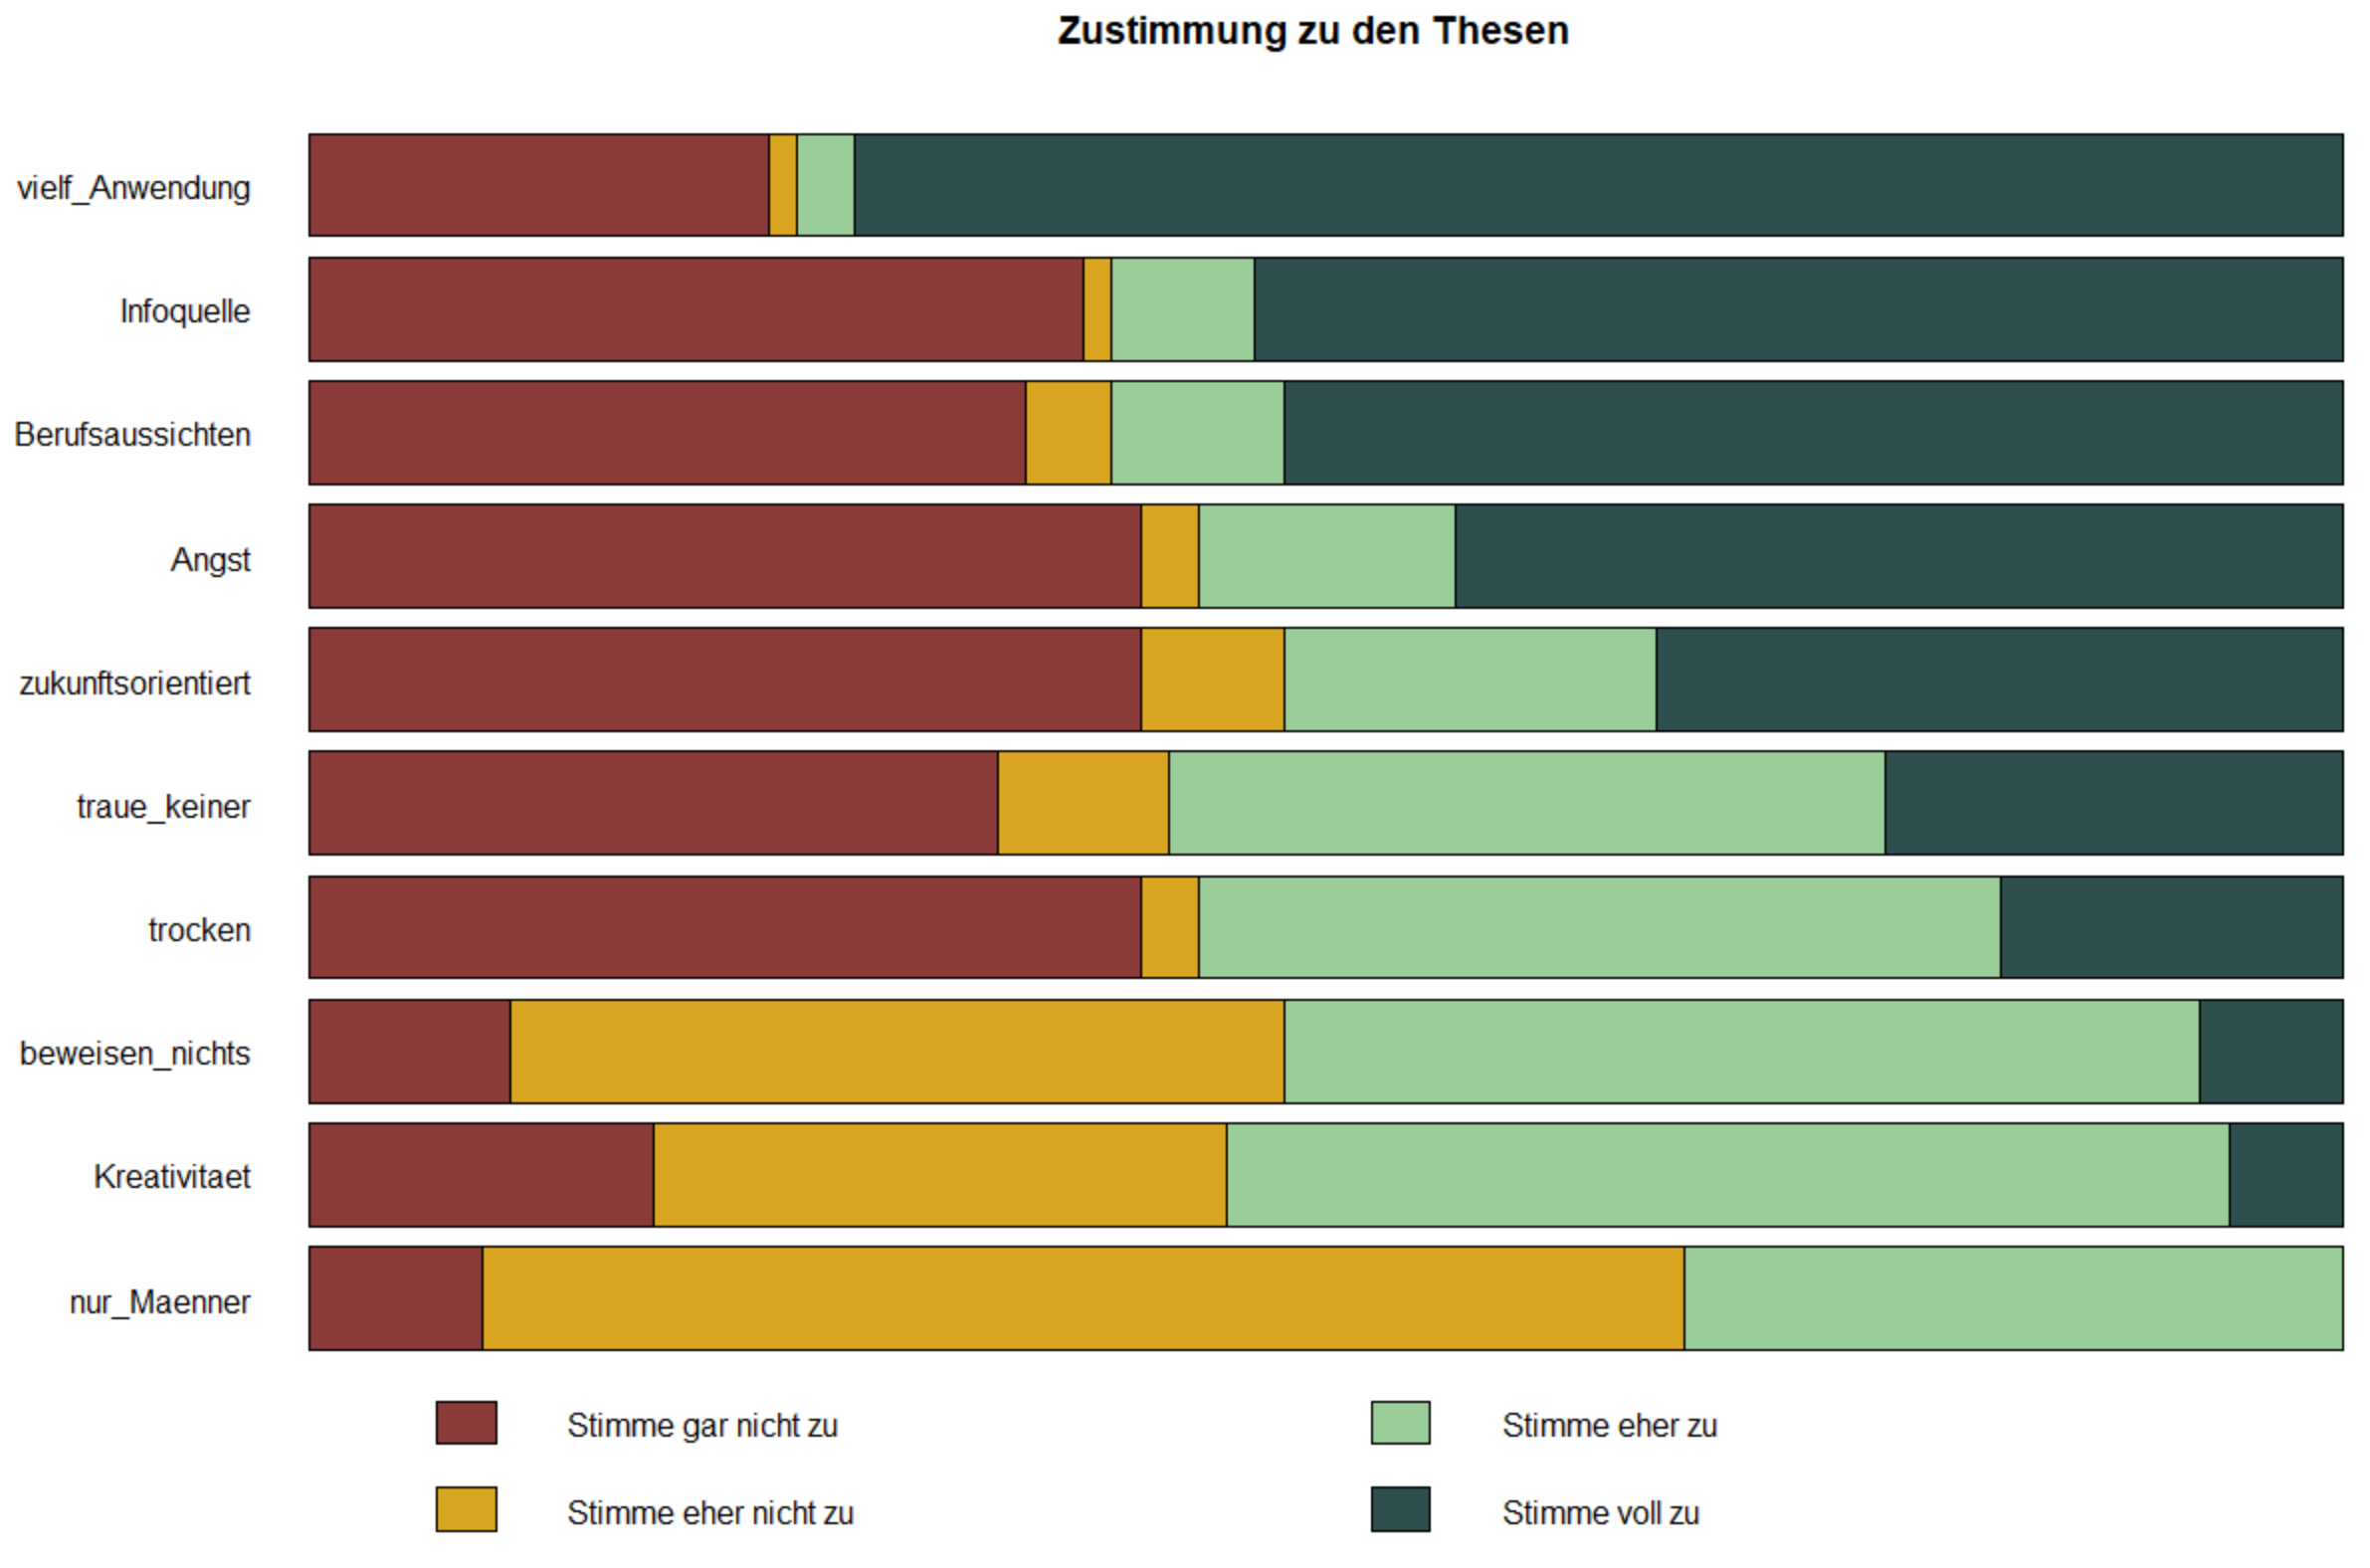
\includegraphics[scale=0.5]{gestapelter_Barplot_Thesen}
\vspace{0.2cm}

%Eigenschaften:
%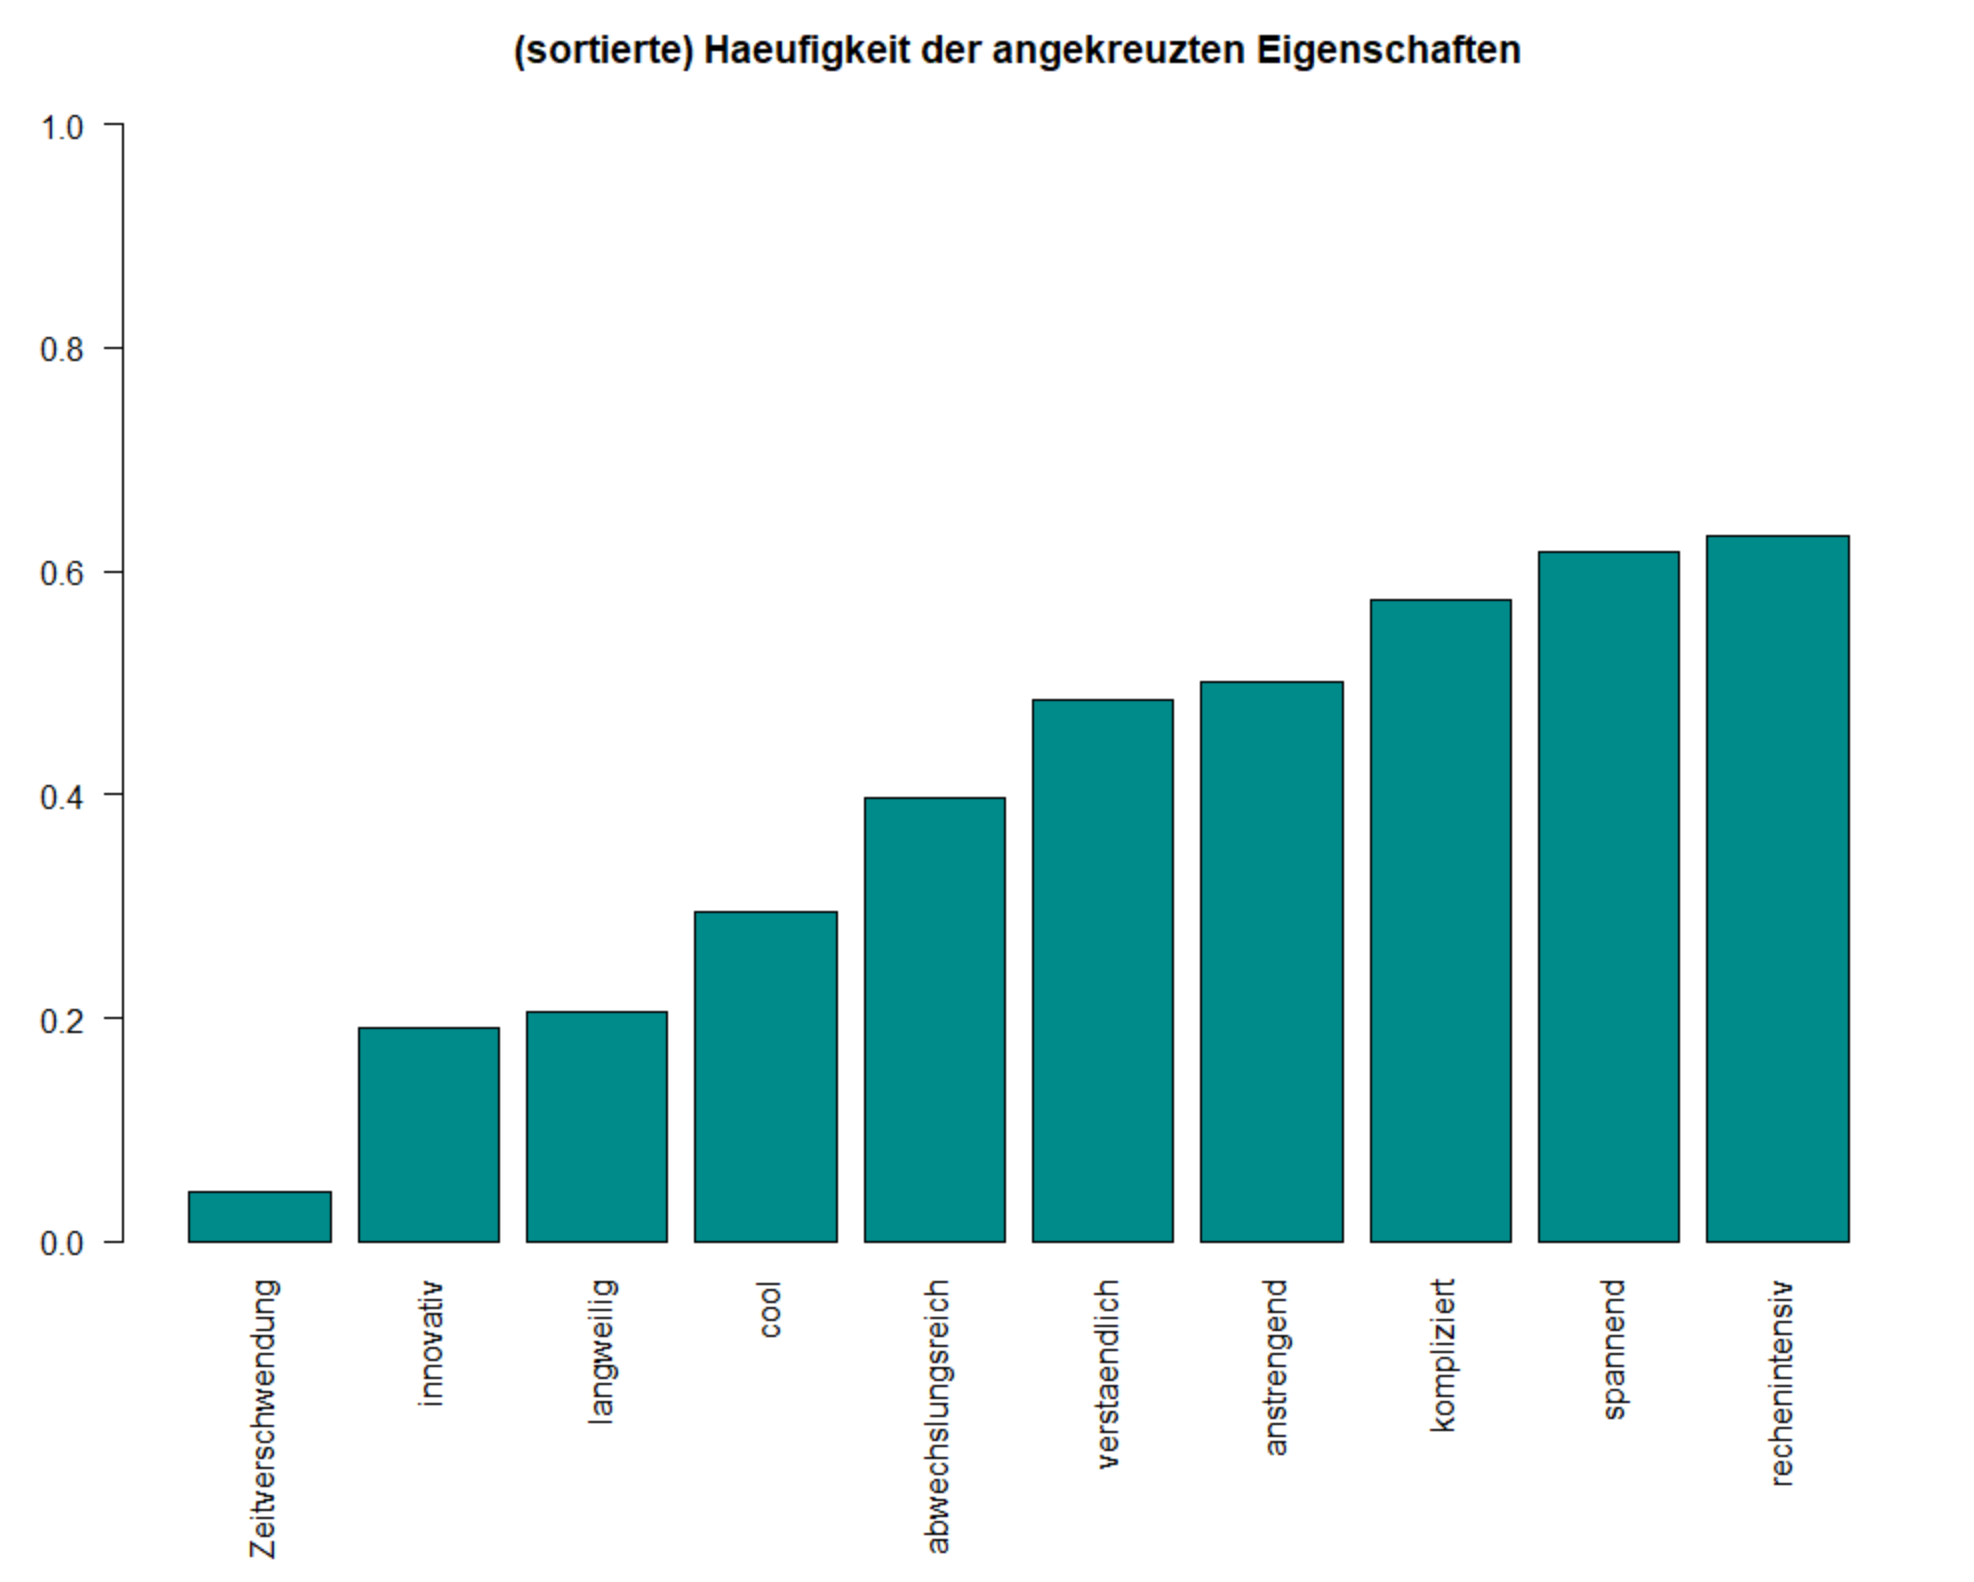
\includegraphics[scale=0.5]{sort_Hfgkeit_angekreuzter_Eigenschaften}
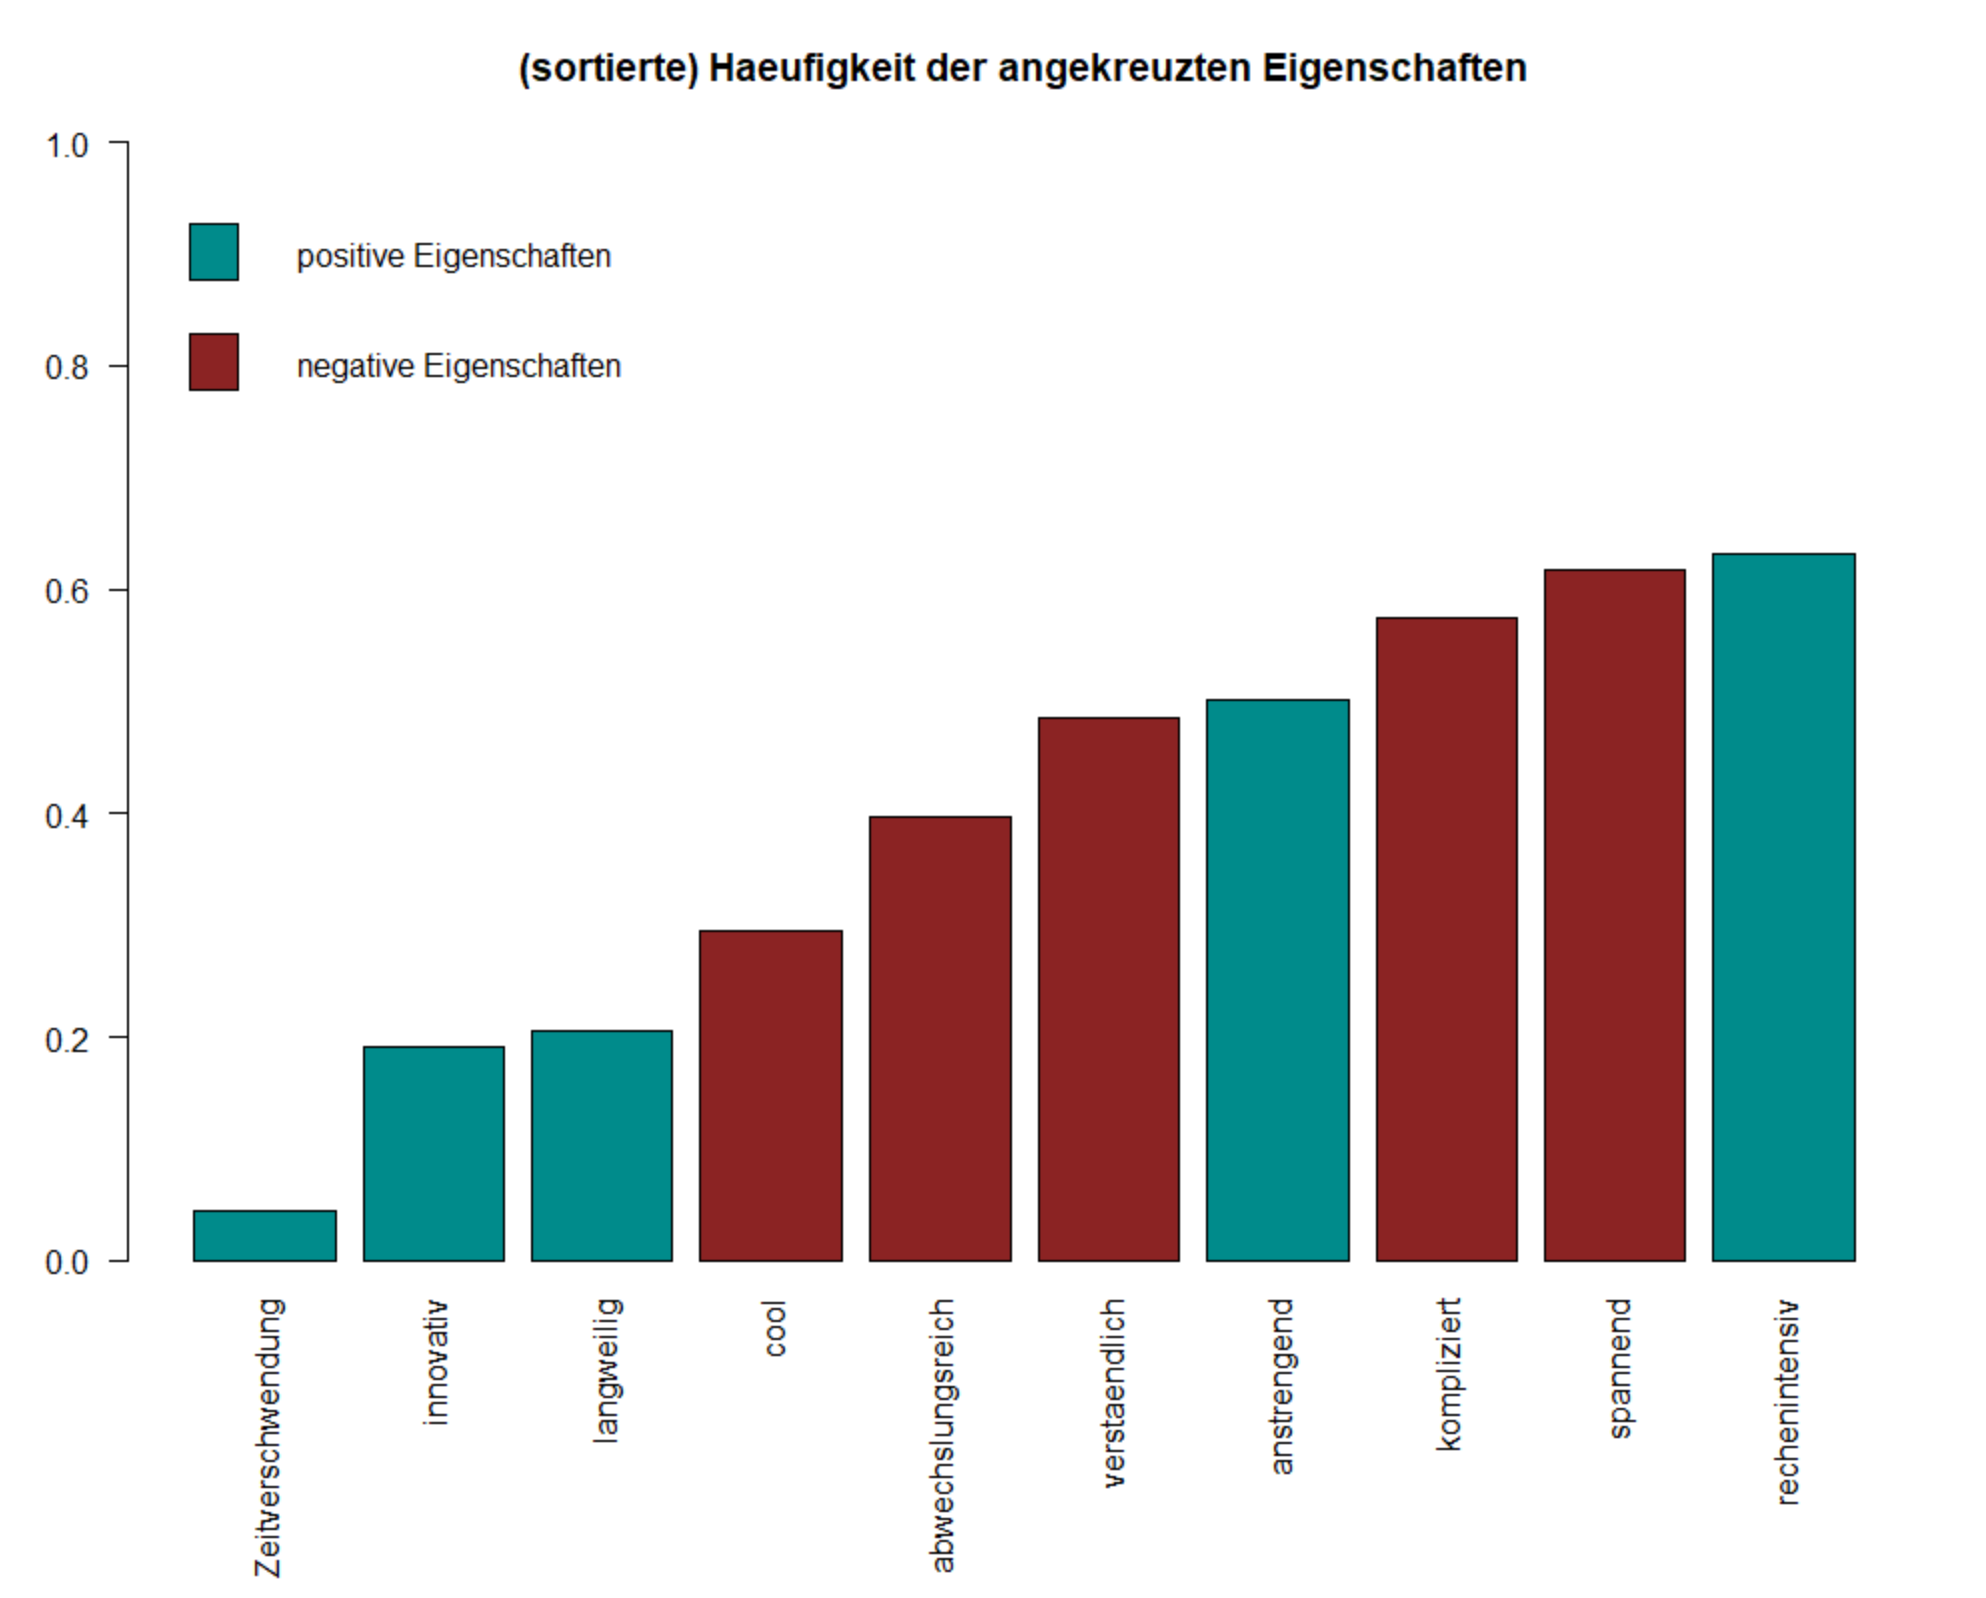
\includegraphics[scale=0.48]{sort_pos_neg_Hfgkeit_angekreuzter_Eigenschaften}\\	
%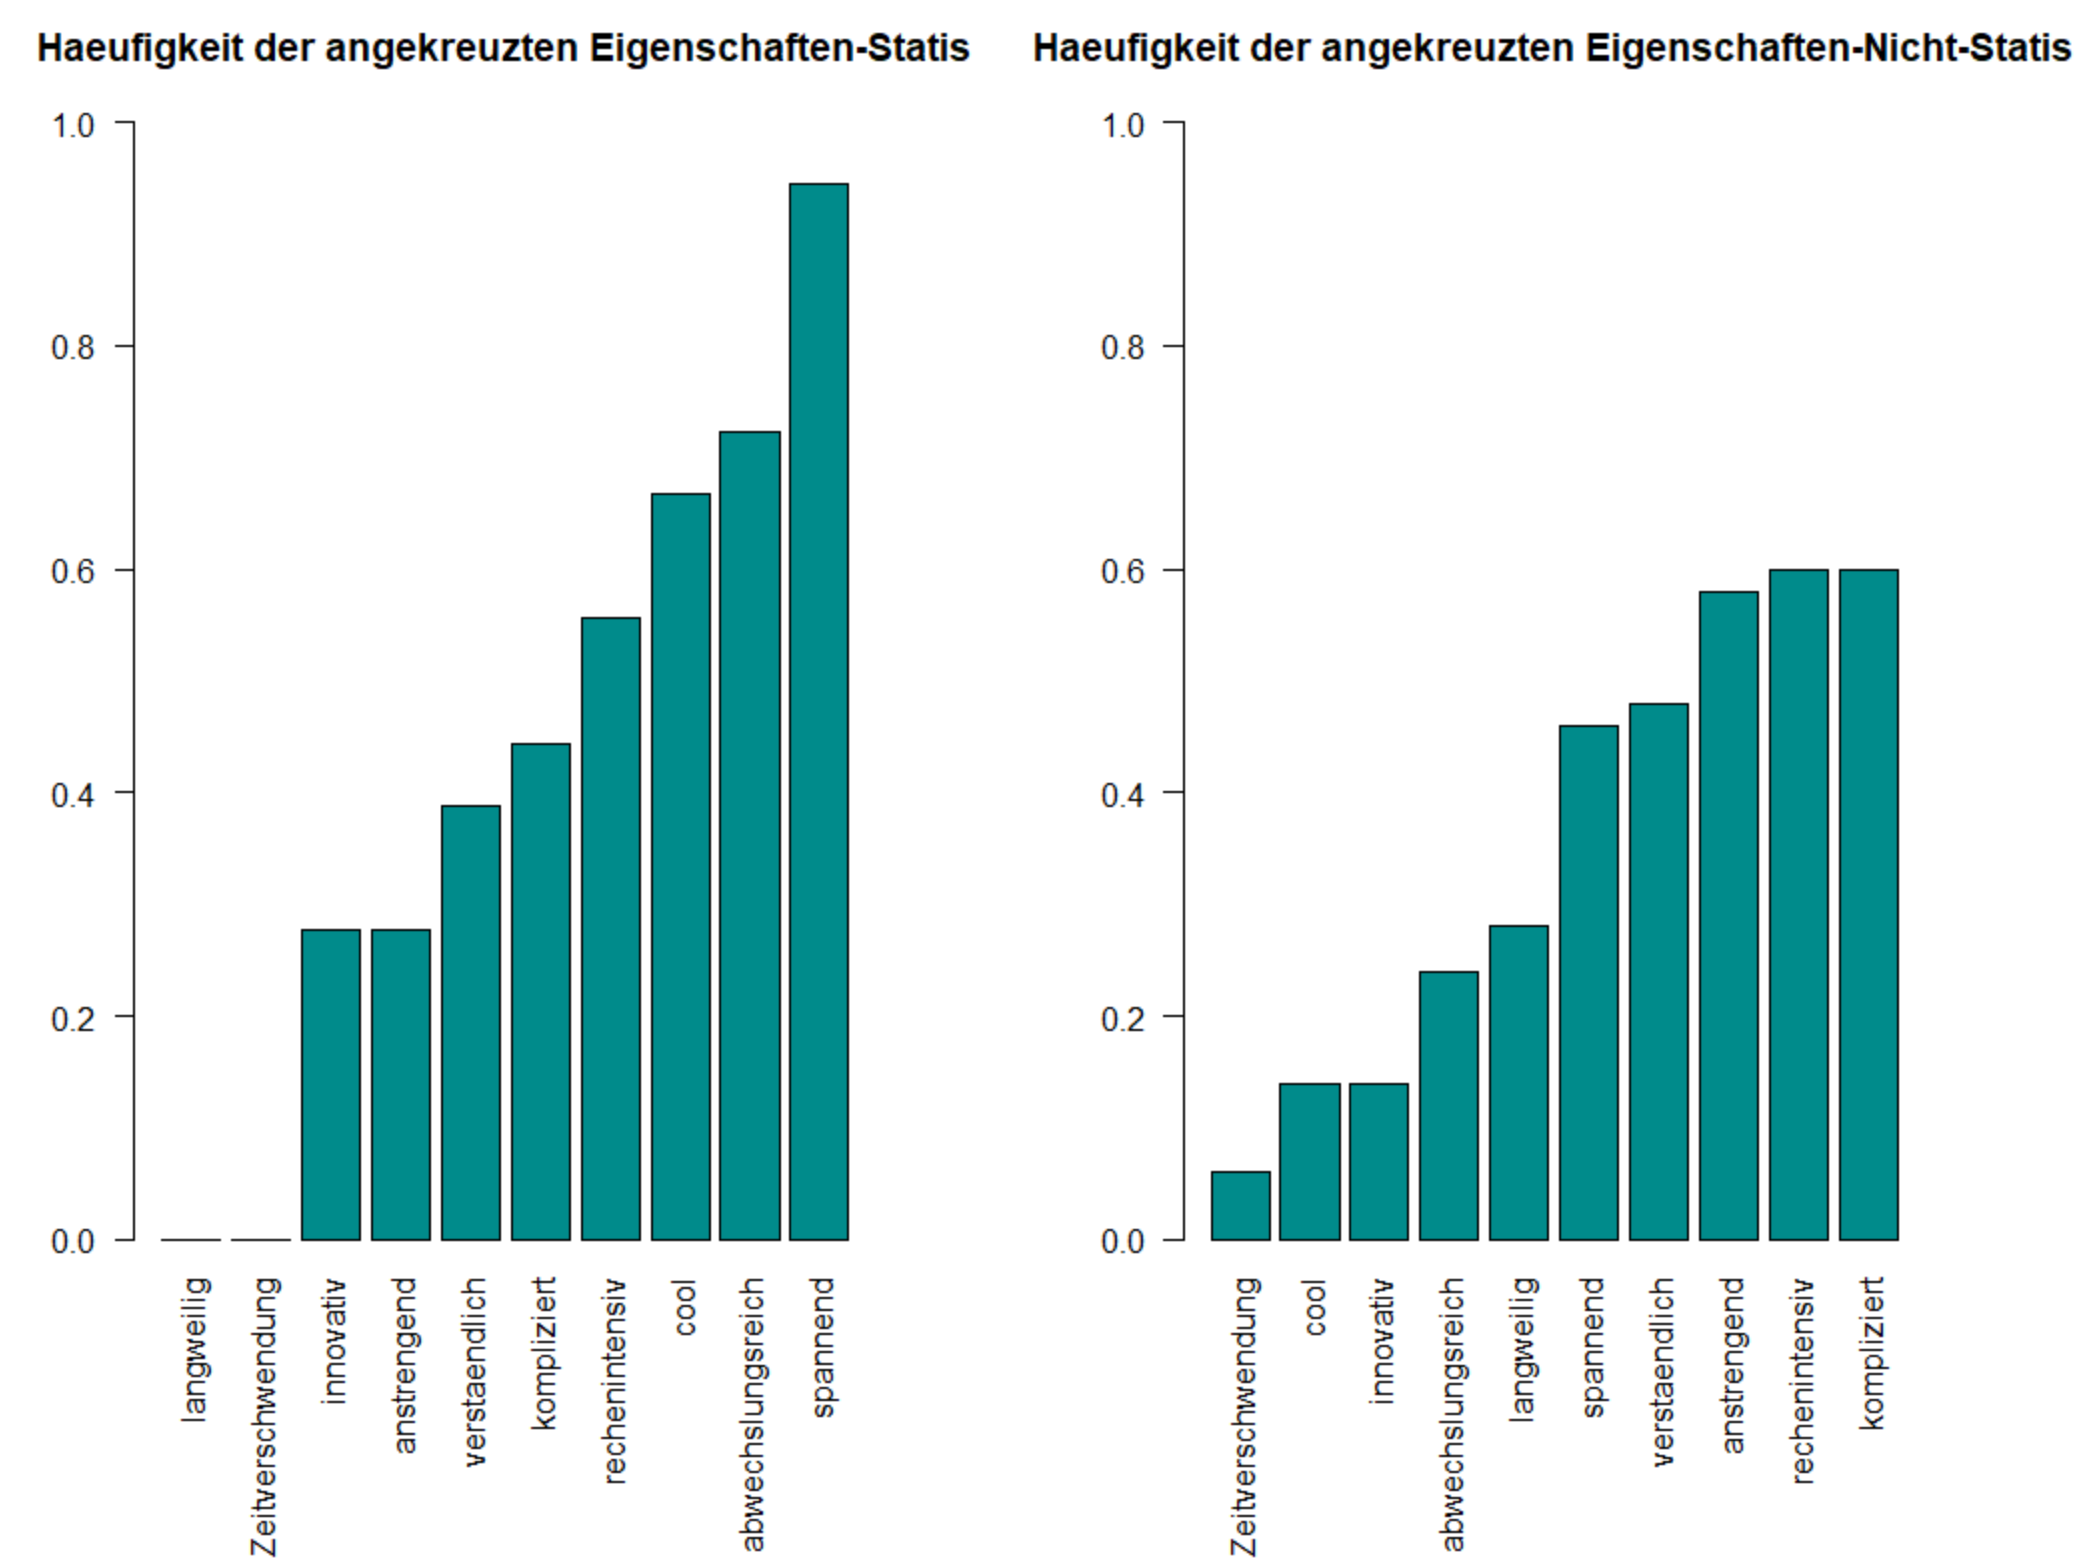
\includegraphics[scale=0.5]{(nicht)-statis_sort_Hfgkeit_angekreuzter_Eigenschaften}
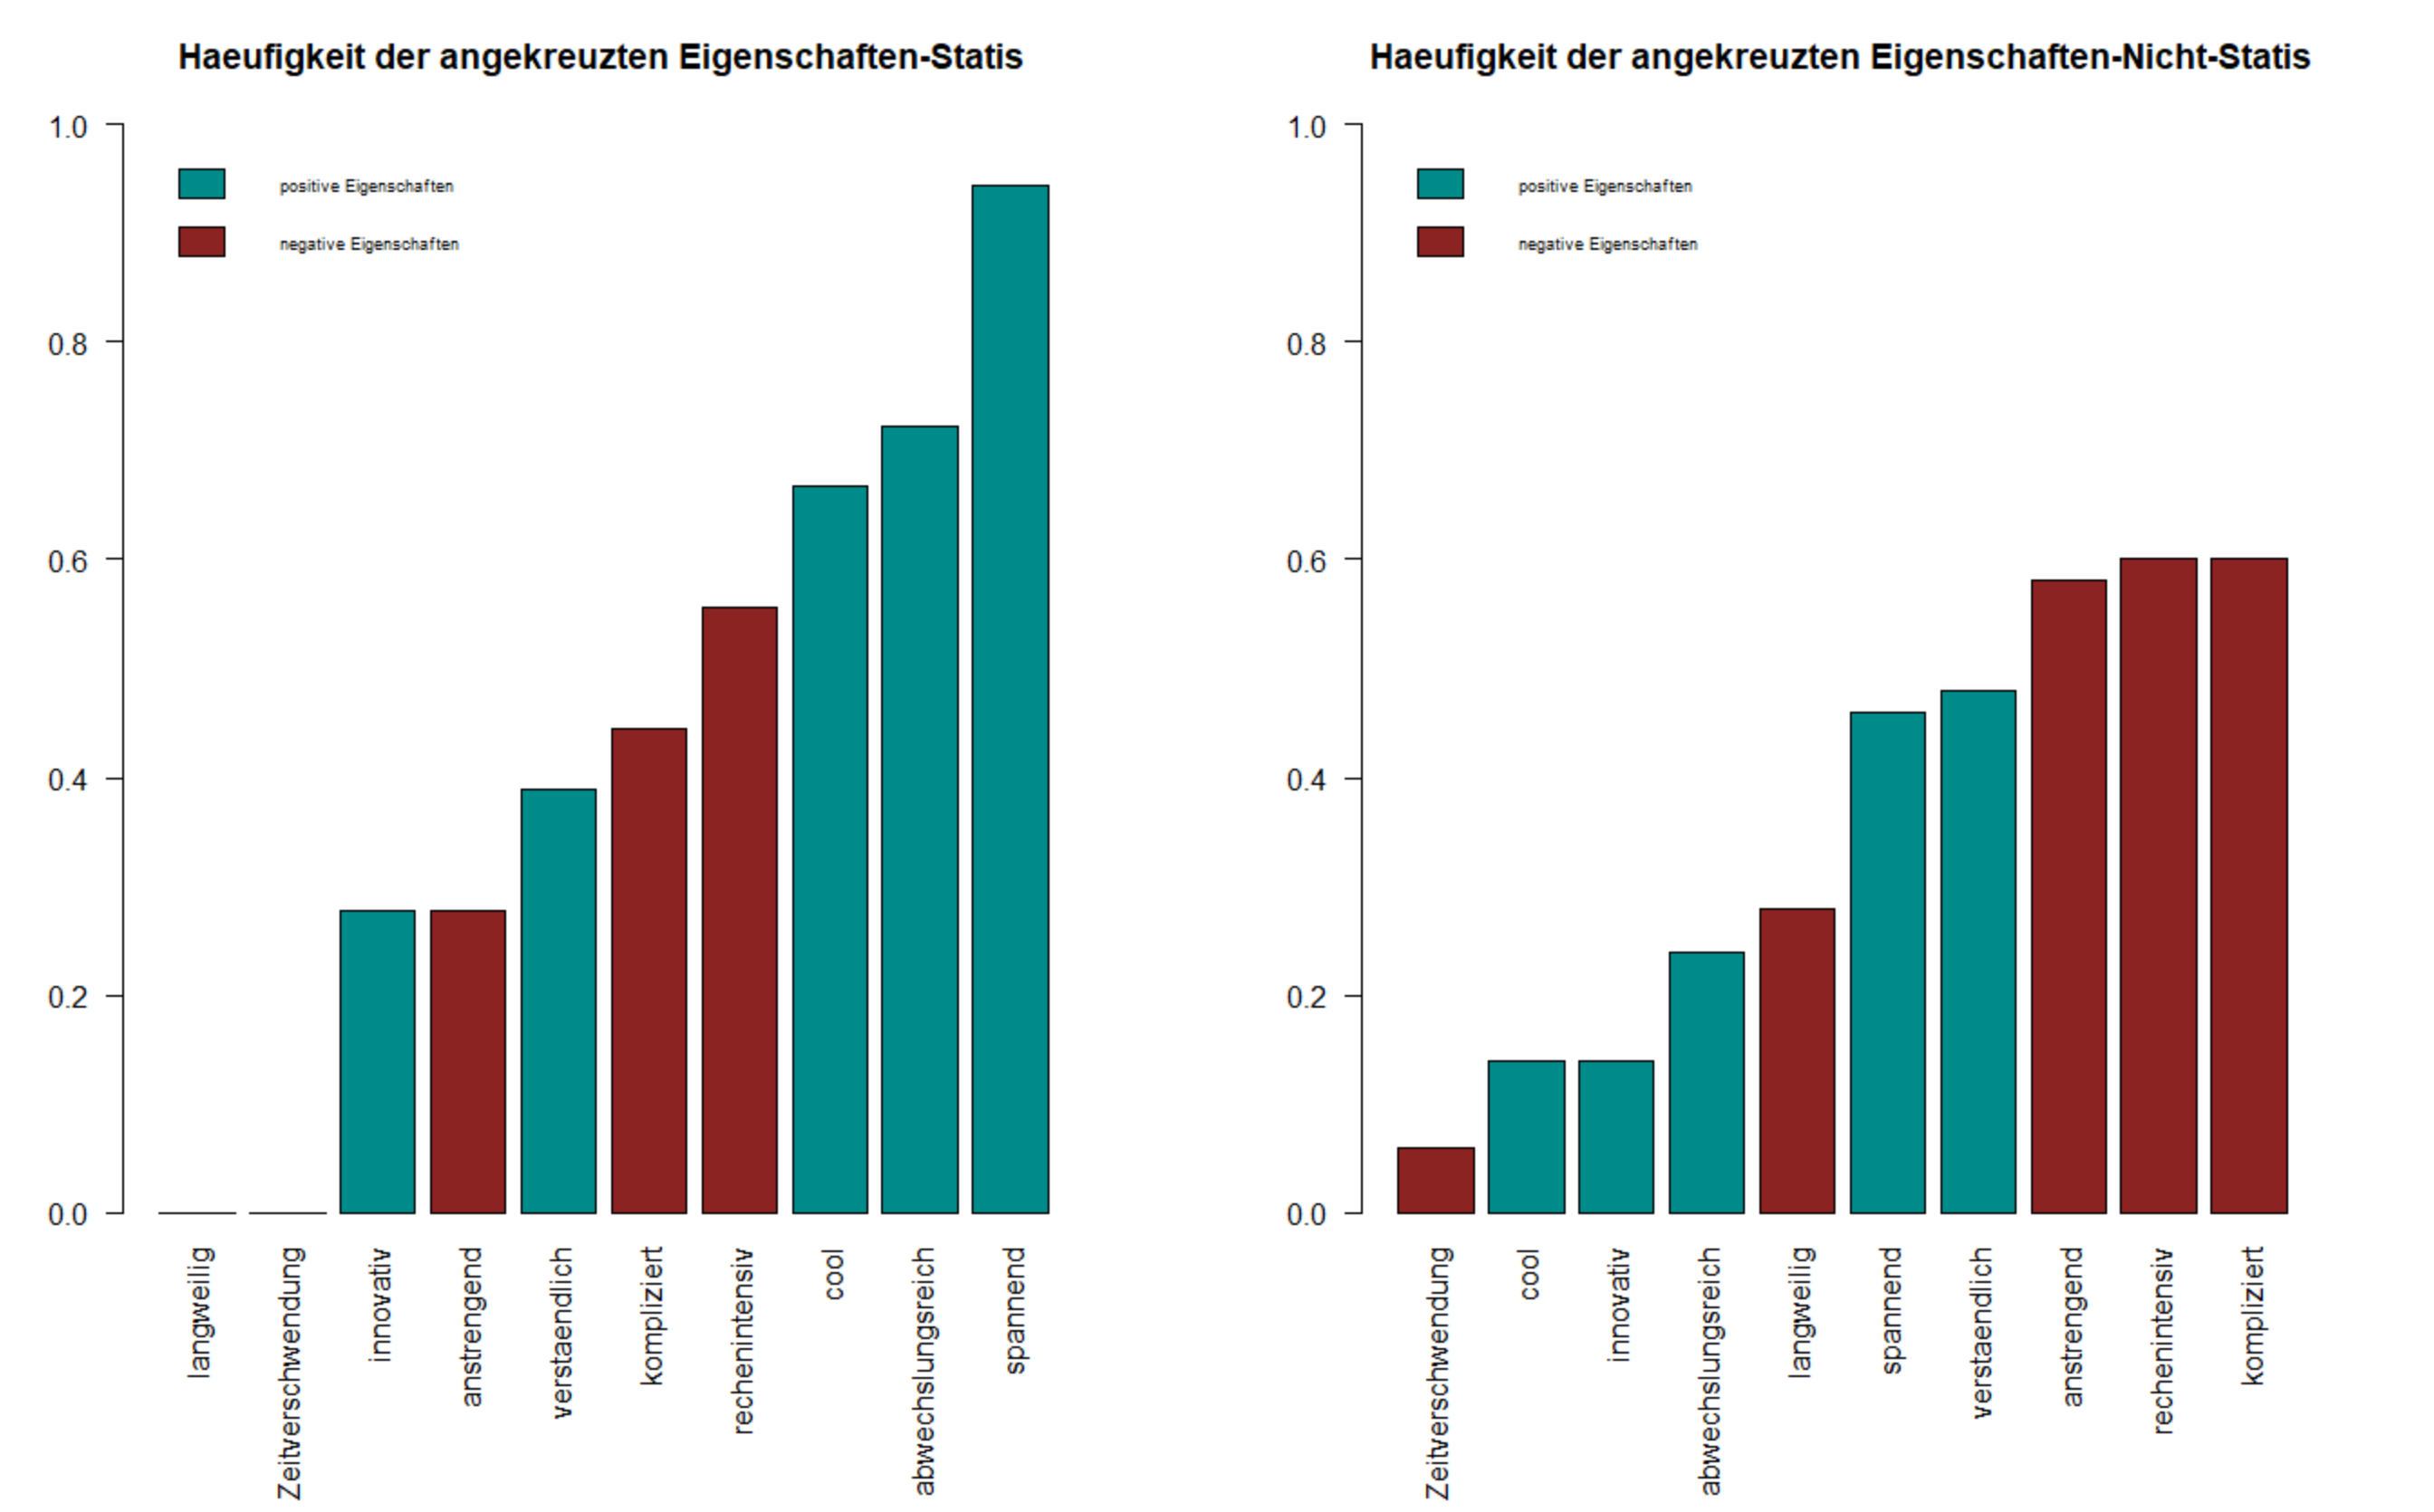
\includegraphics[scale=0.5]{(nicht)-statis_sort_pos_neg_Hfgkeit_angekreuzter_Eigenschaften}\\
\vspace{0.2cm}\\
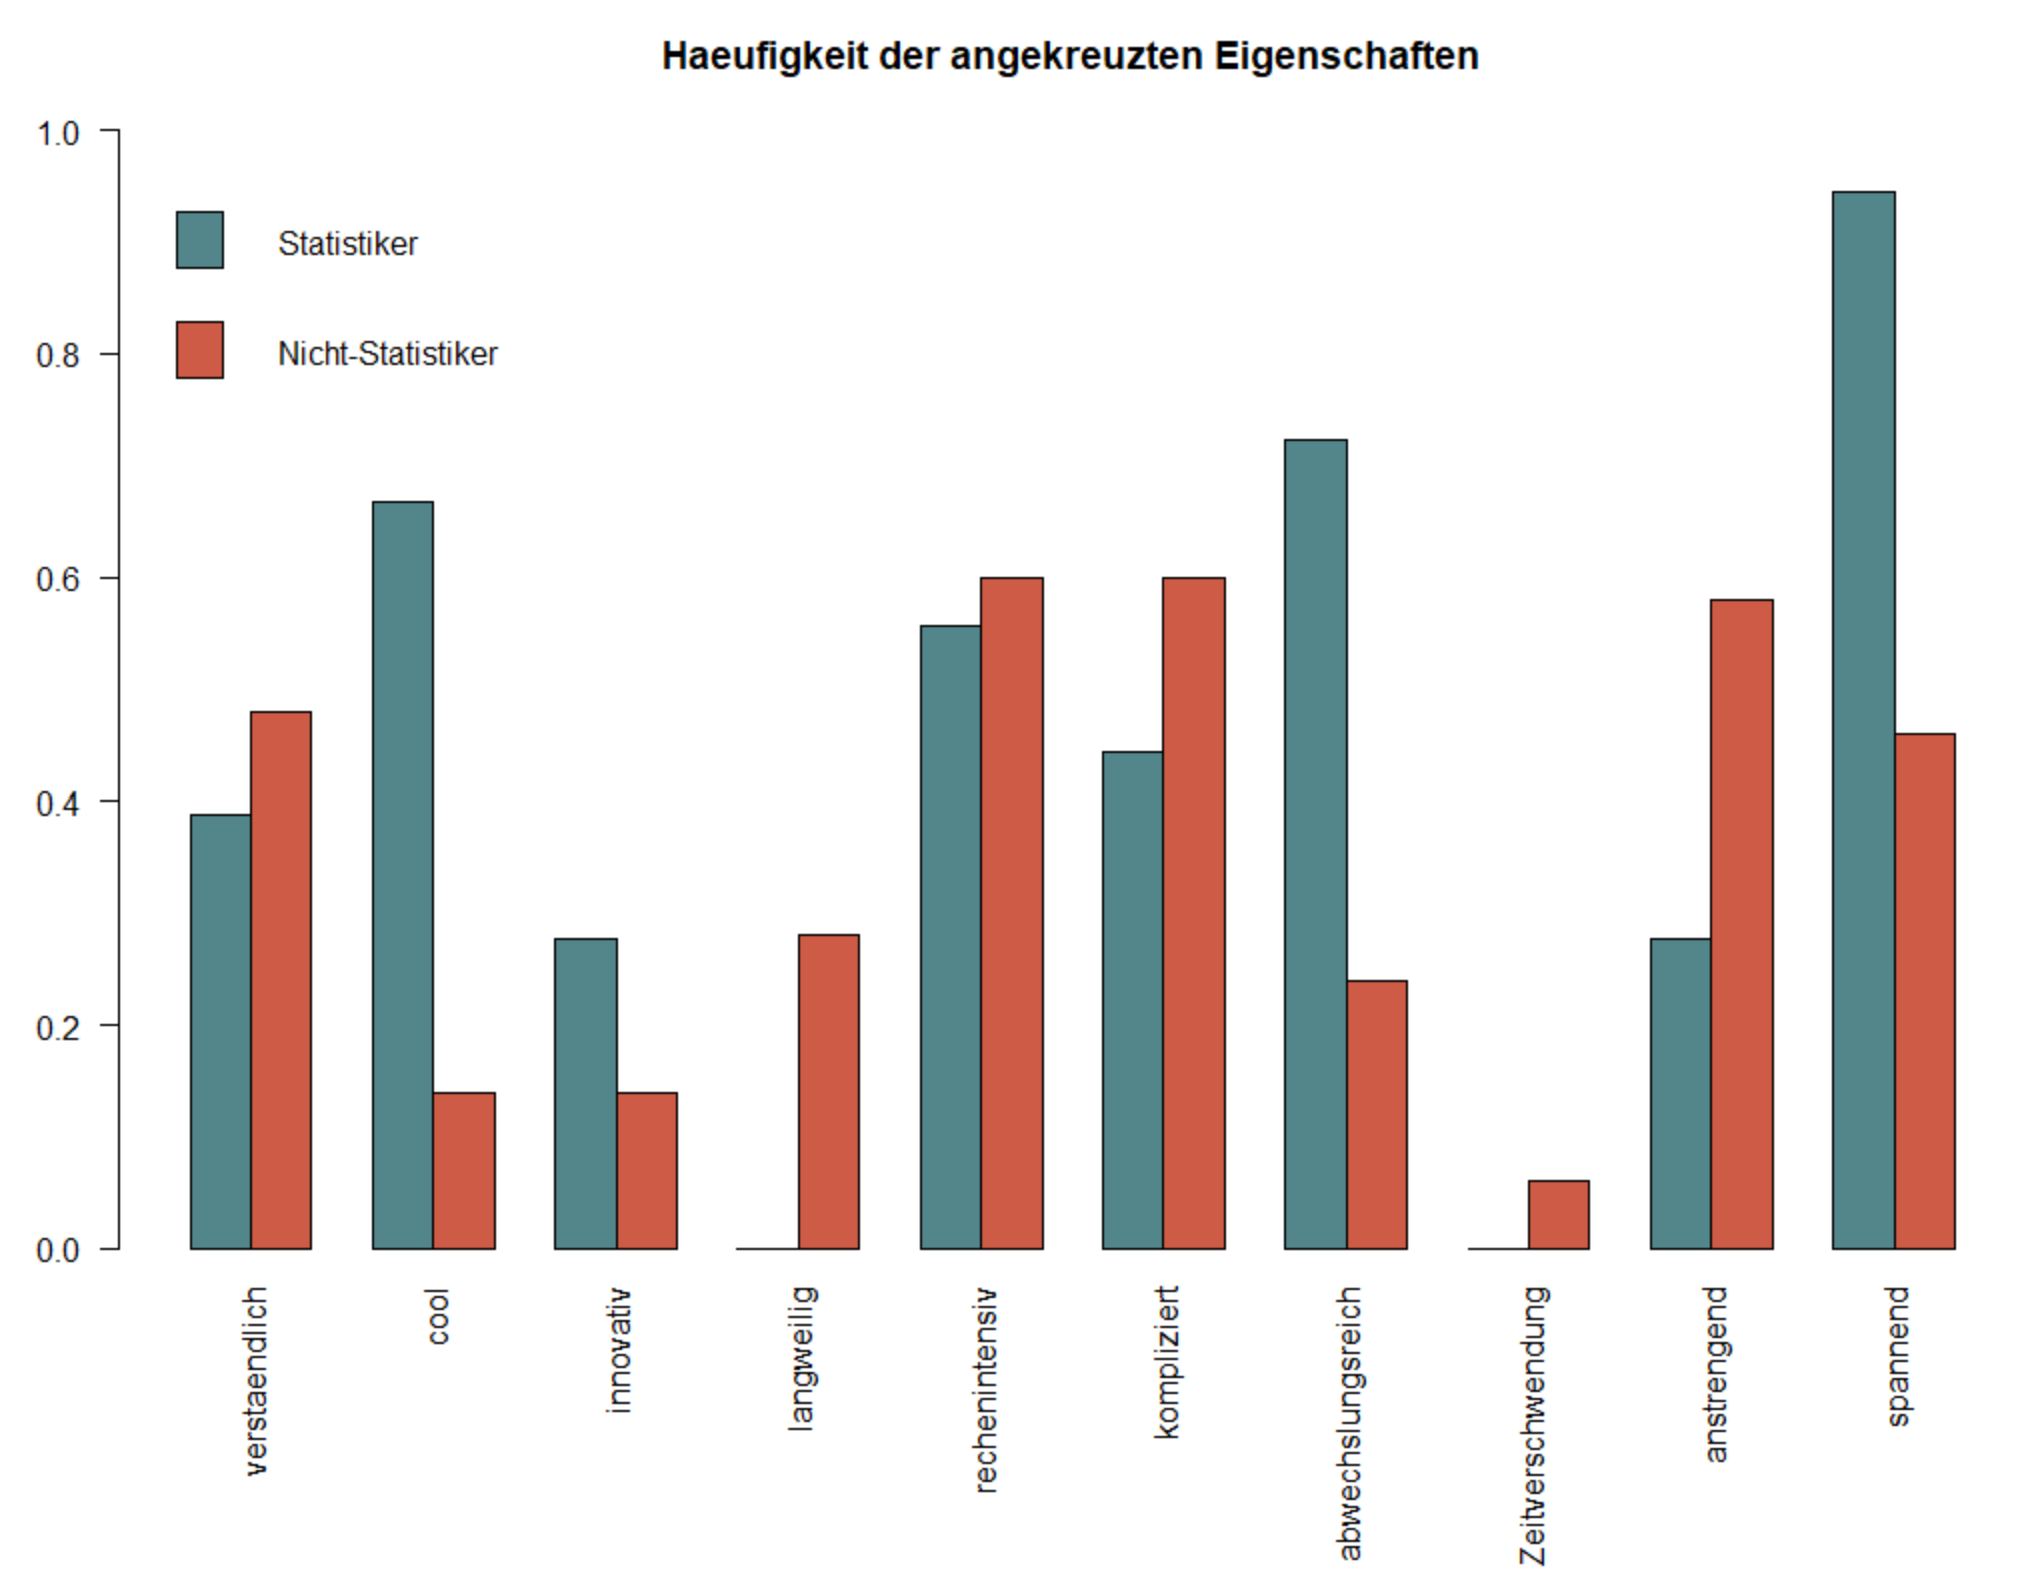
\includegraphics[scale=0.5]{(nicht)-statis_Hfgkeit_angekreuzter_Eigenschaften}\\


%Relevanz:\\
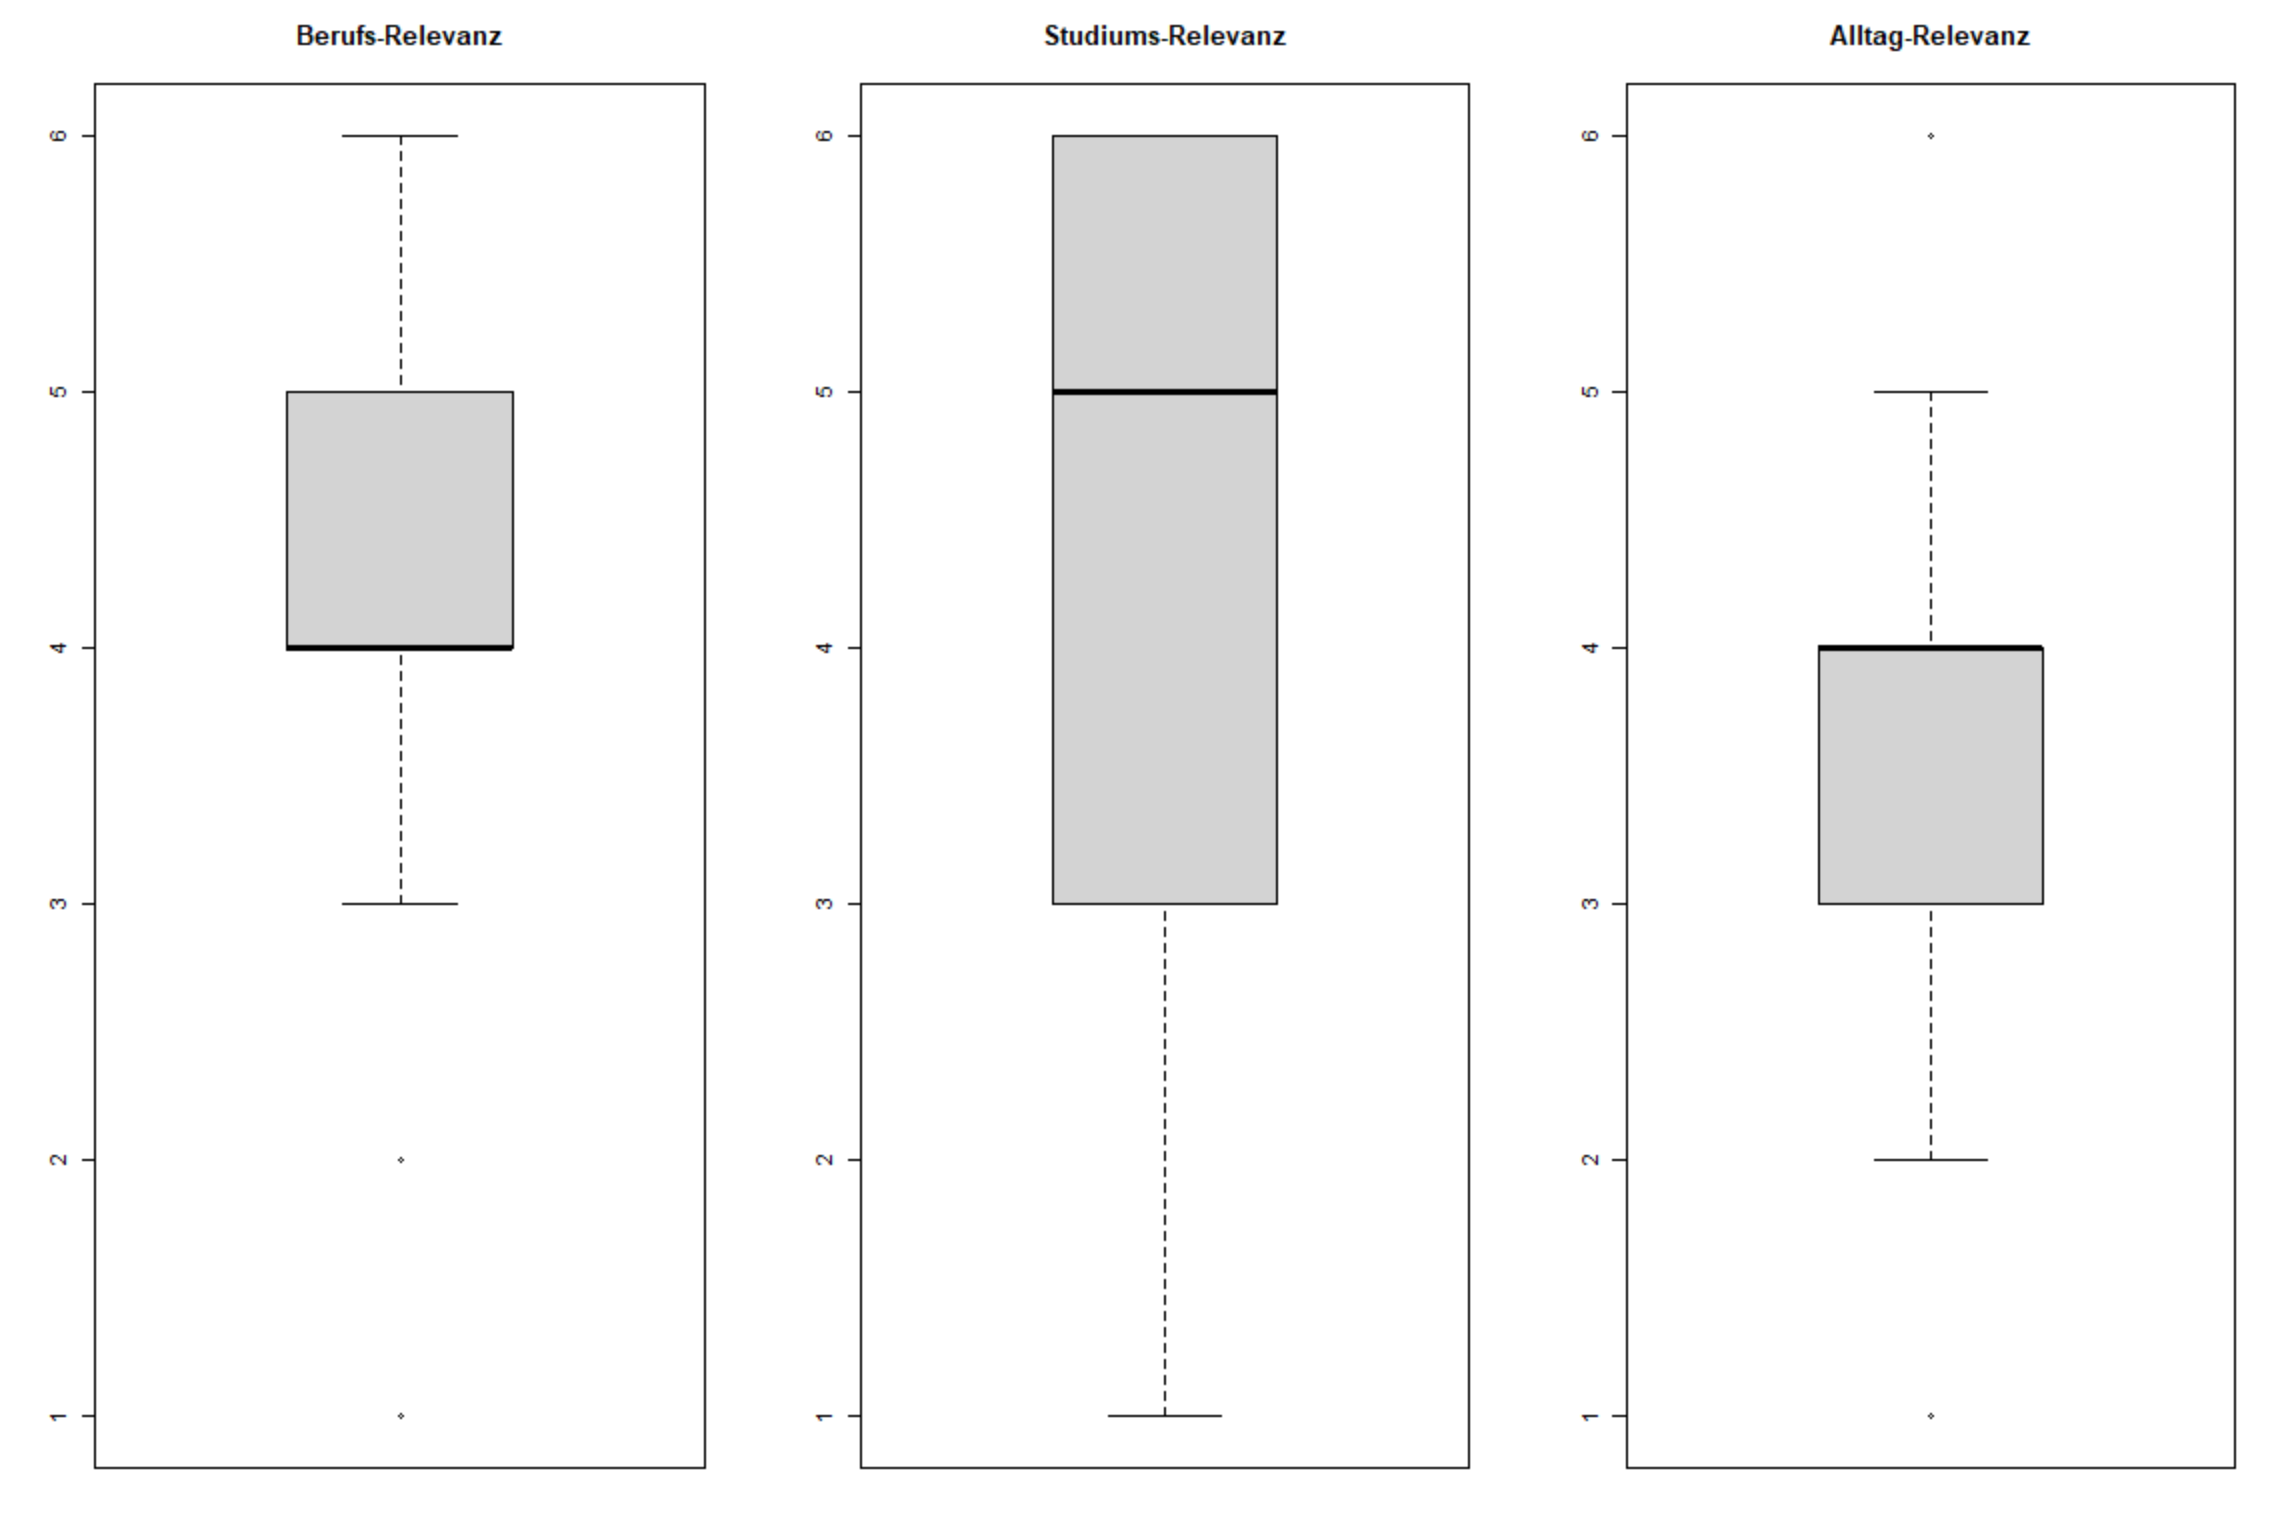
\includegraphics[scale=0.49]{3_boxplots_relevanz}\\
%\vspace{0.1cm}\\
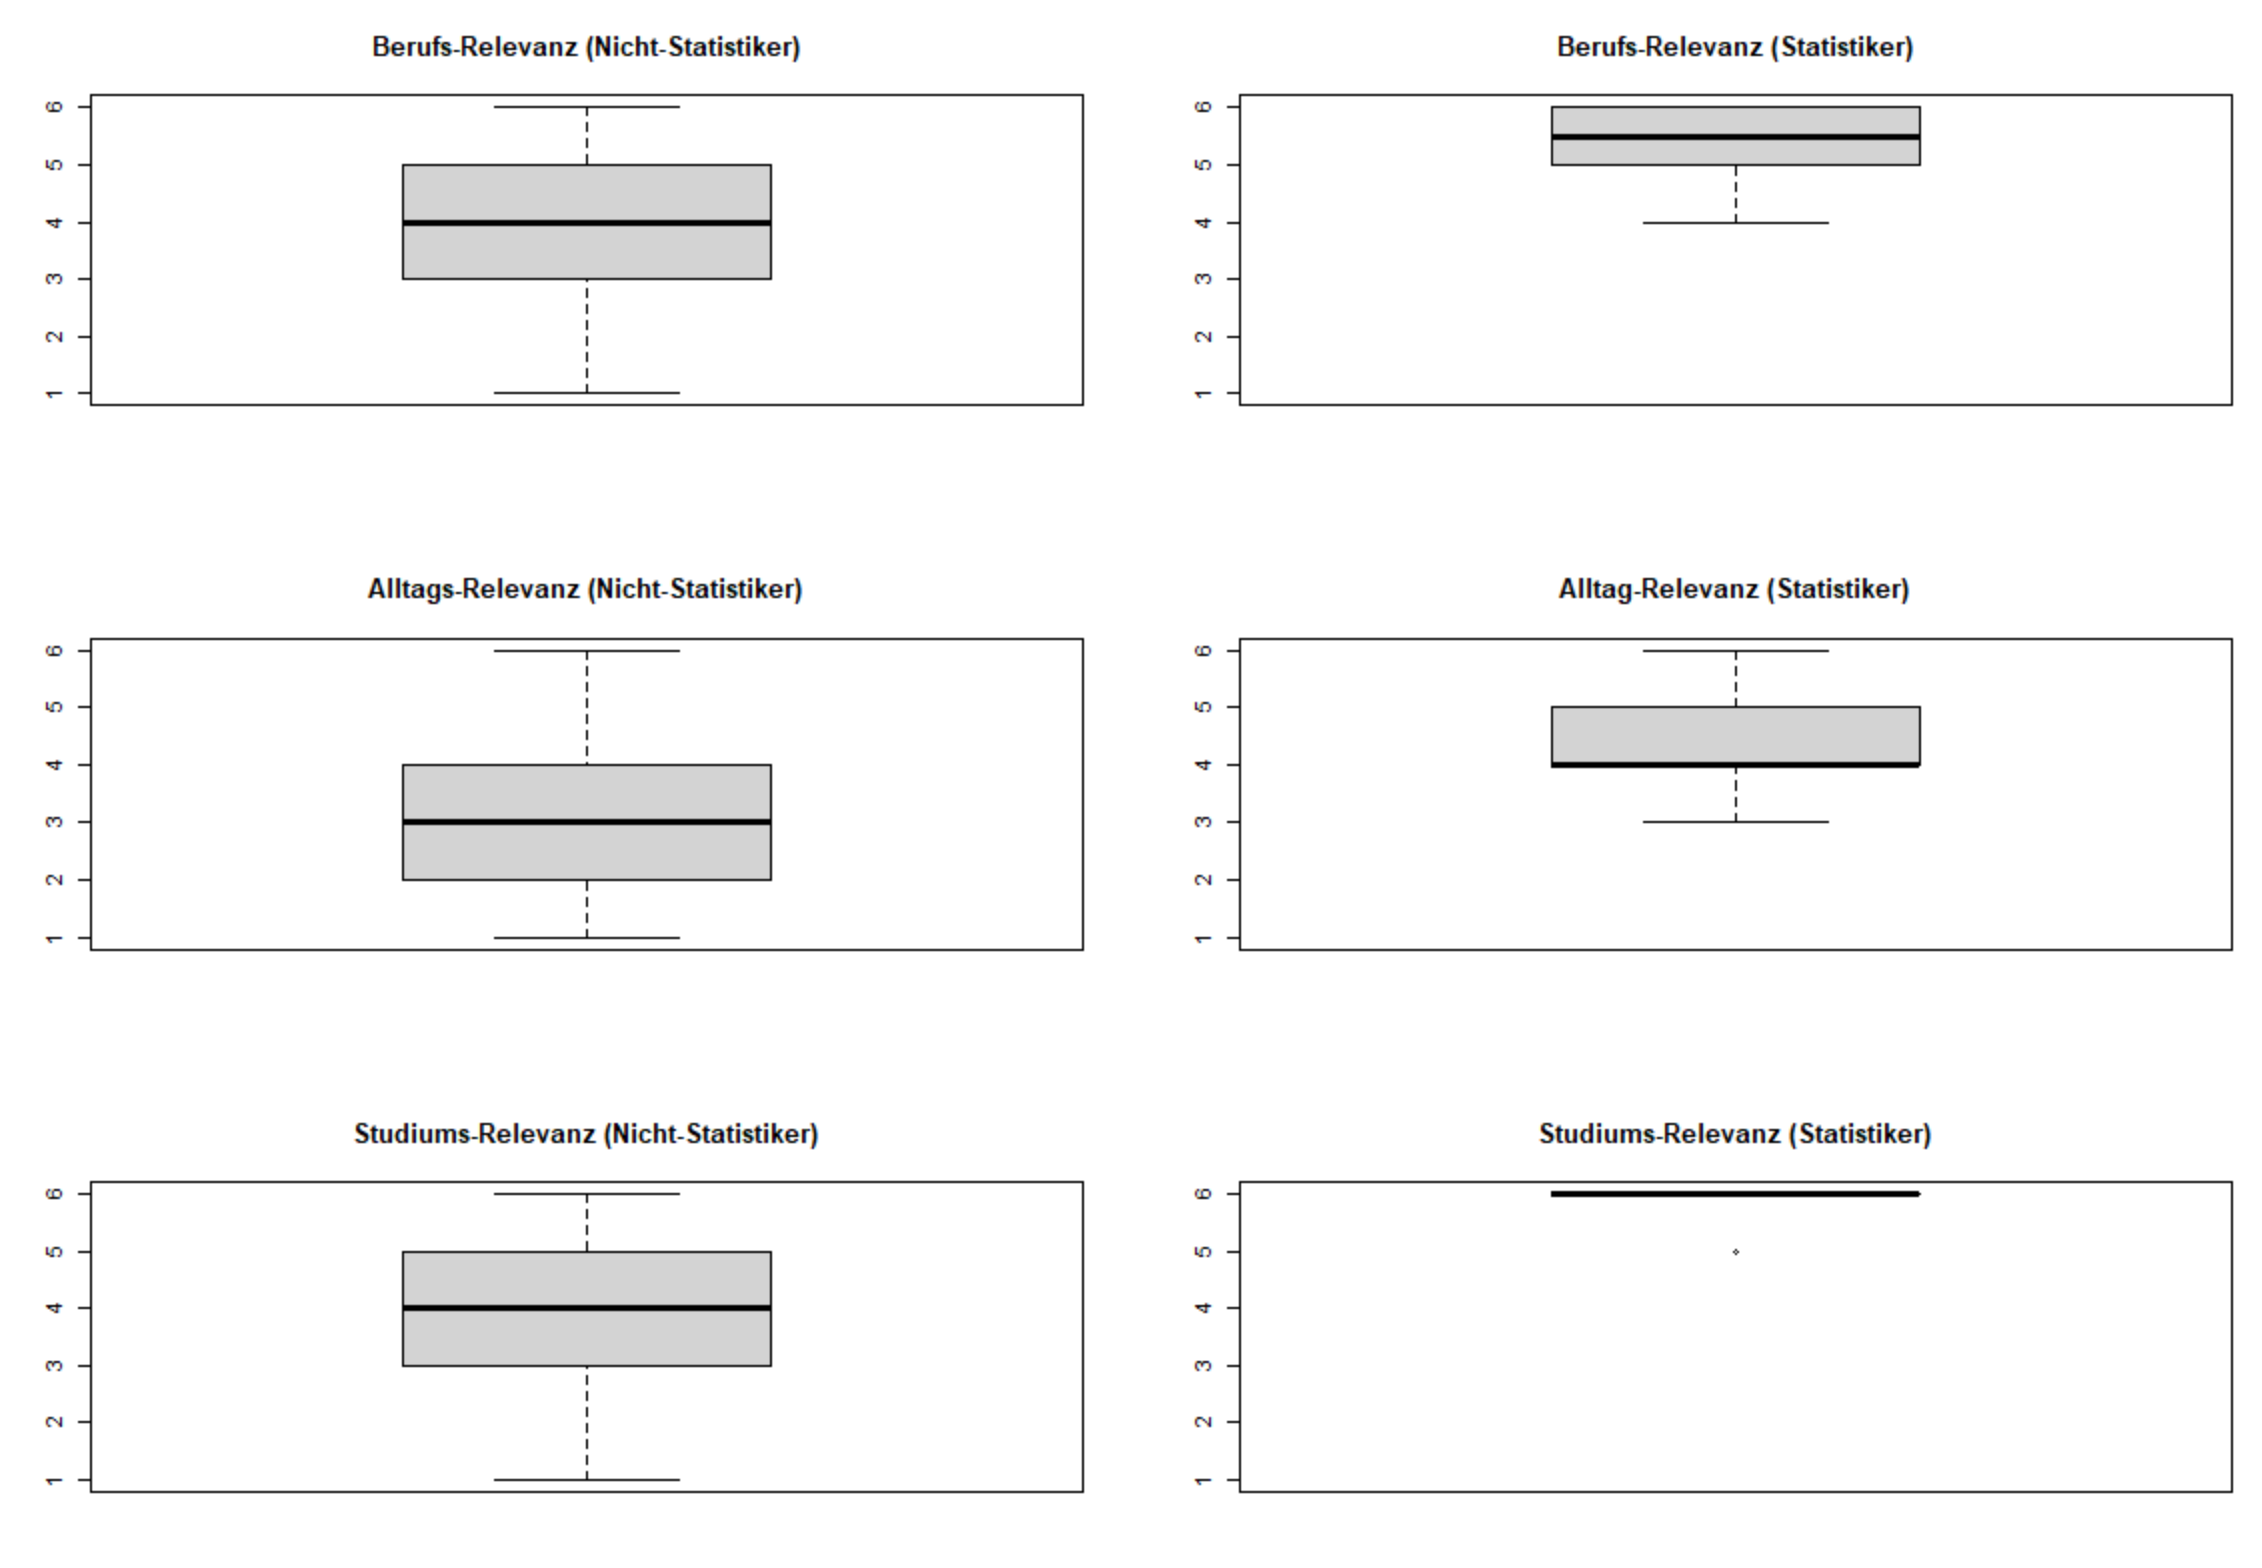
\includegraphics[scale=0.49]{(nicht)-statis_boxplots_Relevanz}\\
{\tiny 1 $=$ Absolut irrelevant, 2 $=$ Ziemlich irrelevant, 3 $=$ Eher irrelevant, 4 $=$ Eher relevant, 5 $=$ Ziemlich relevant, 6 $=$ Absolut relevant}\\


%Assoziationen:\\
\hspace{-2cm}
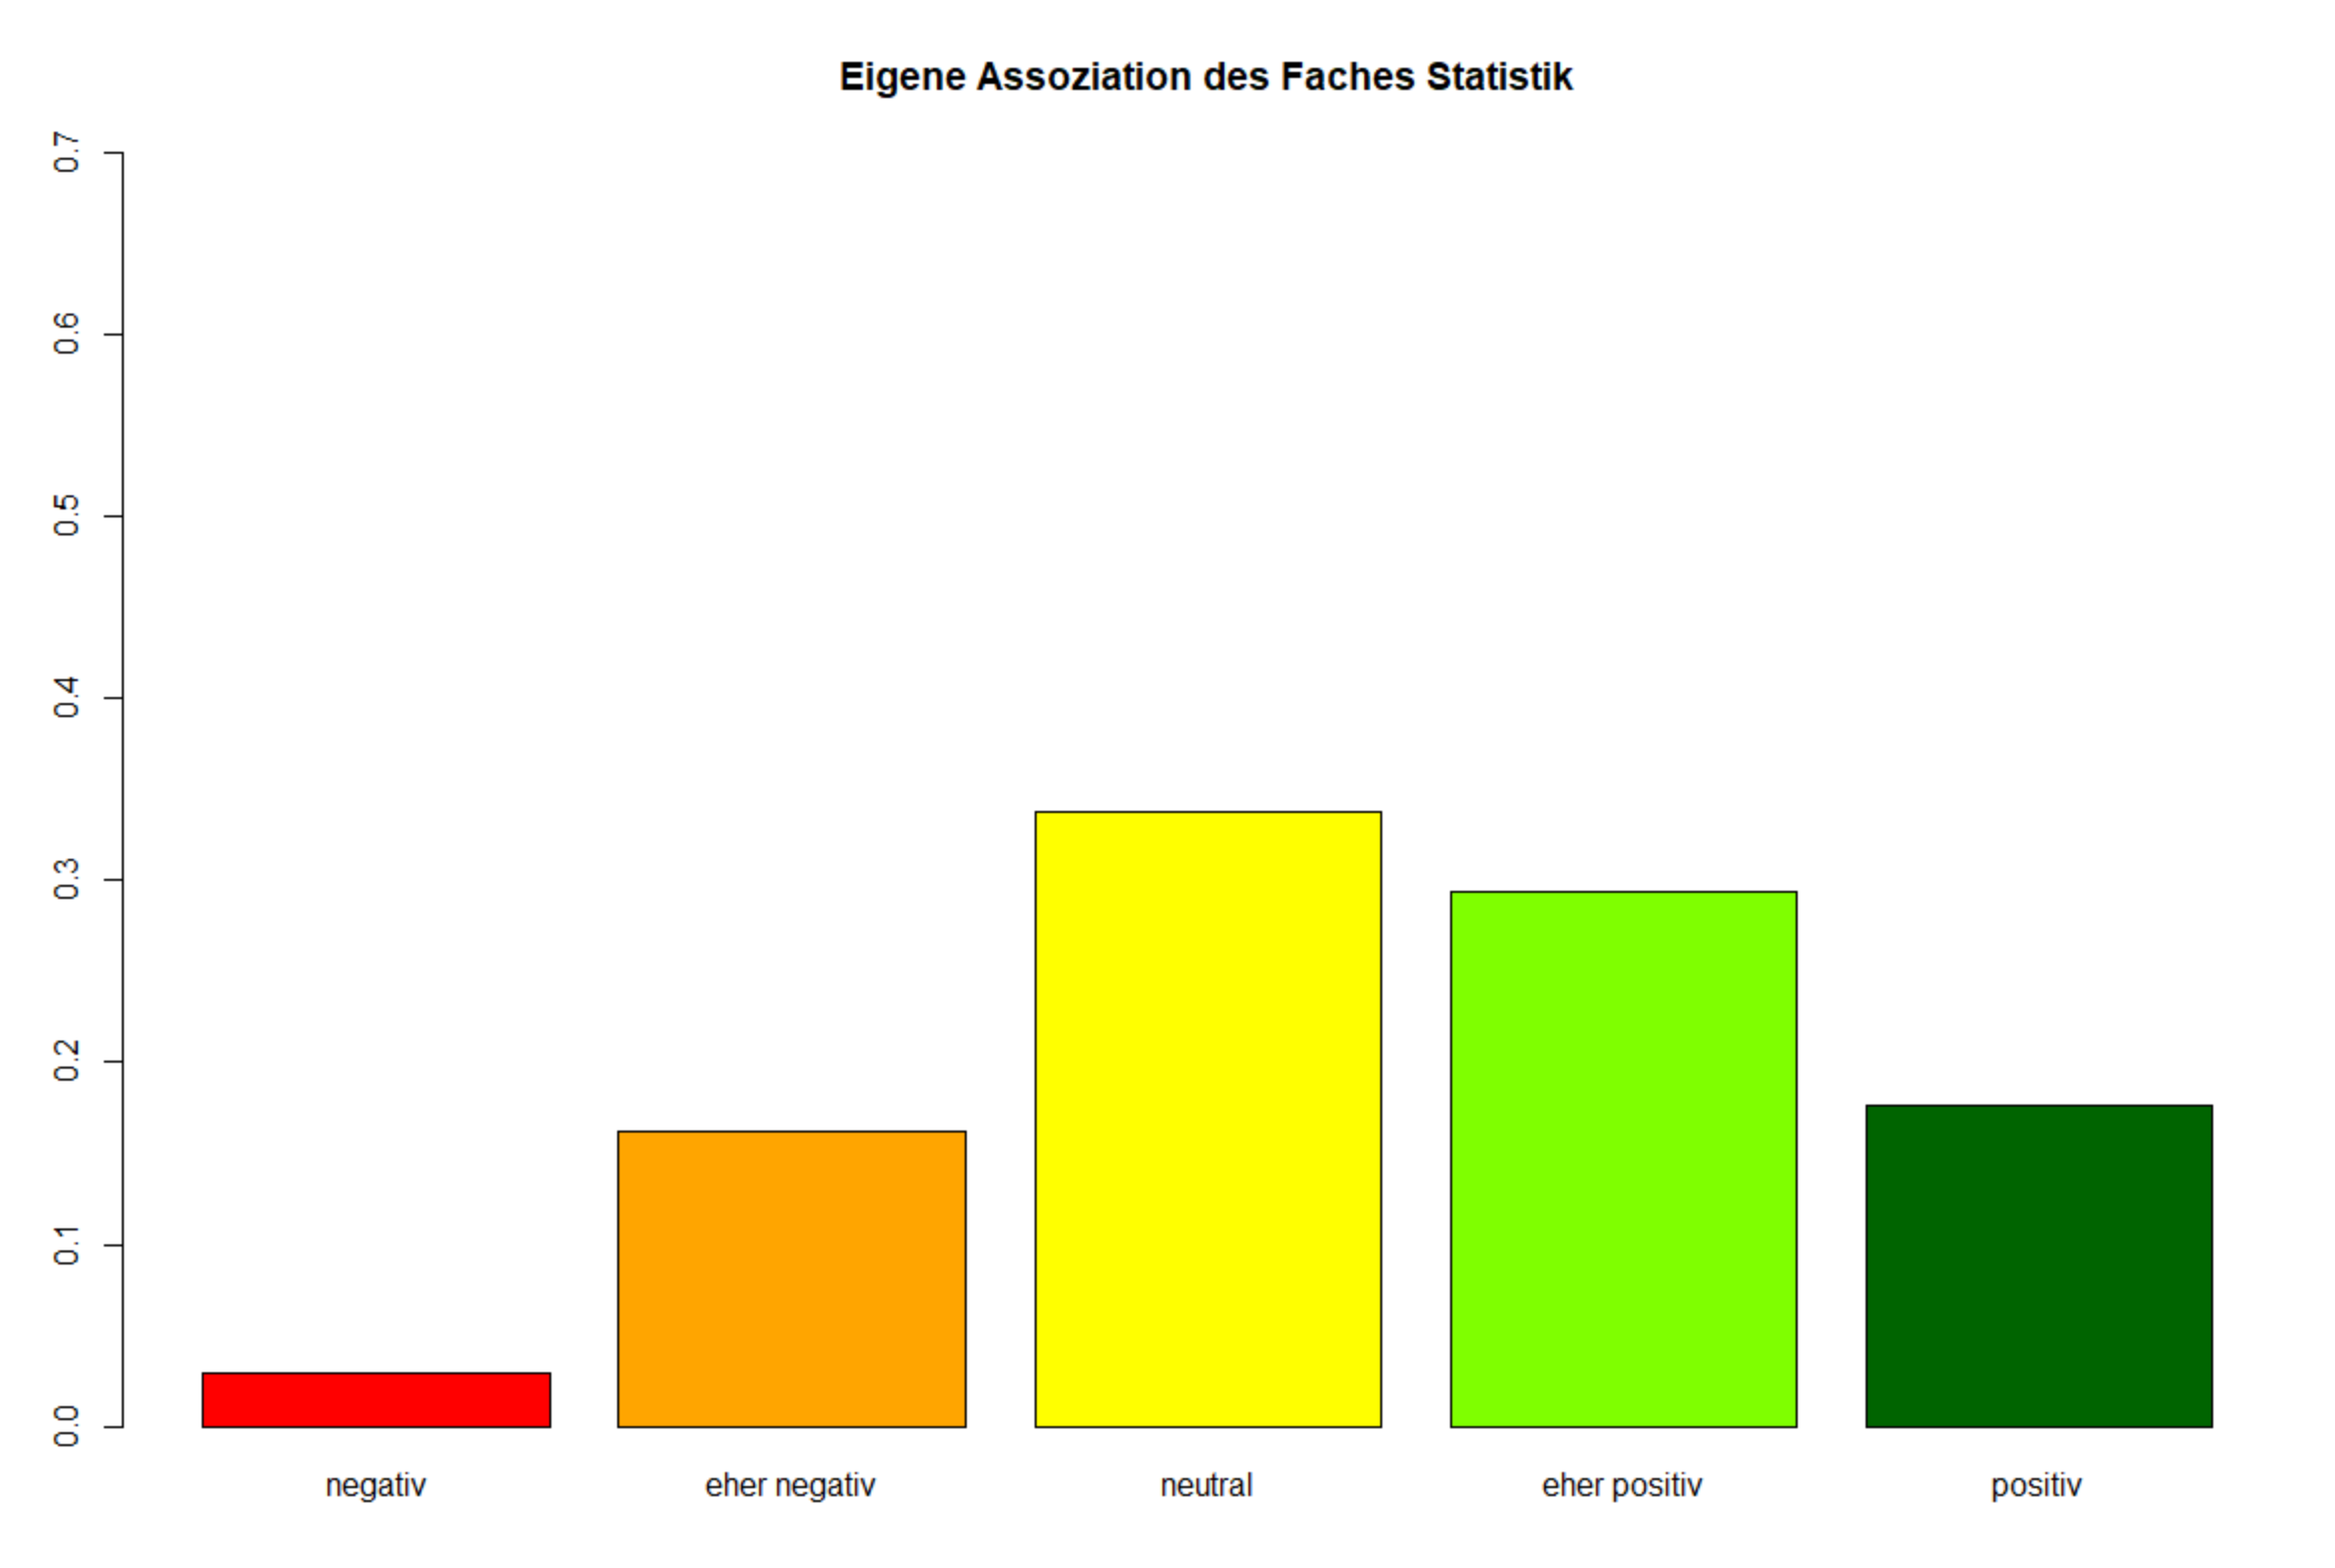
\includegraphics[scale=0.3]{barplot_Assoziation}
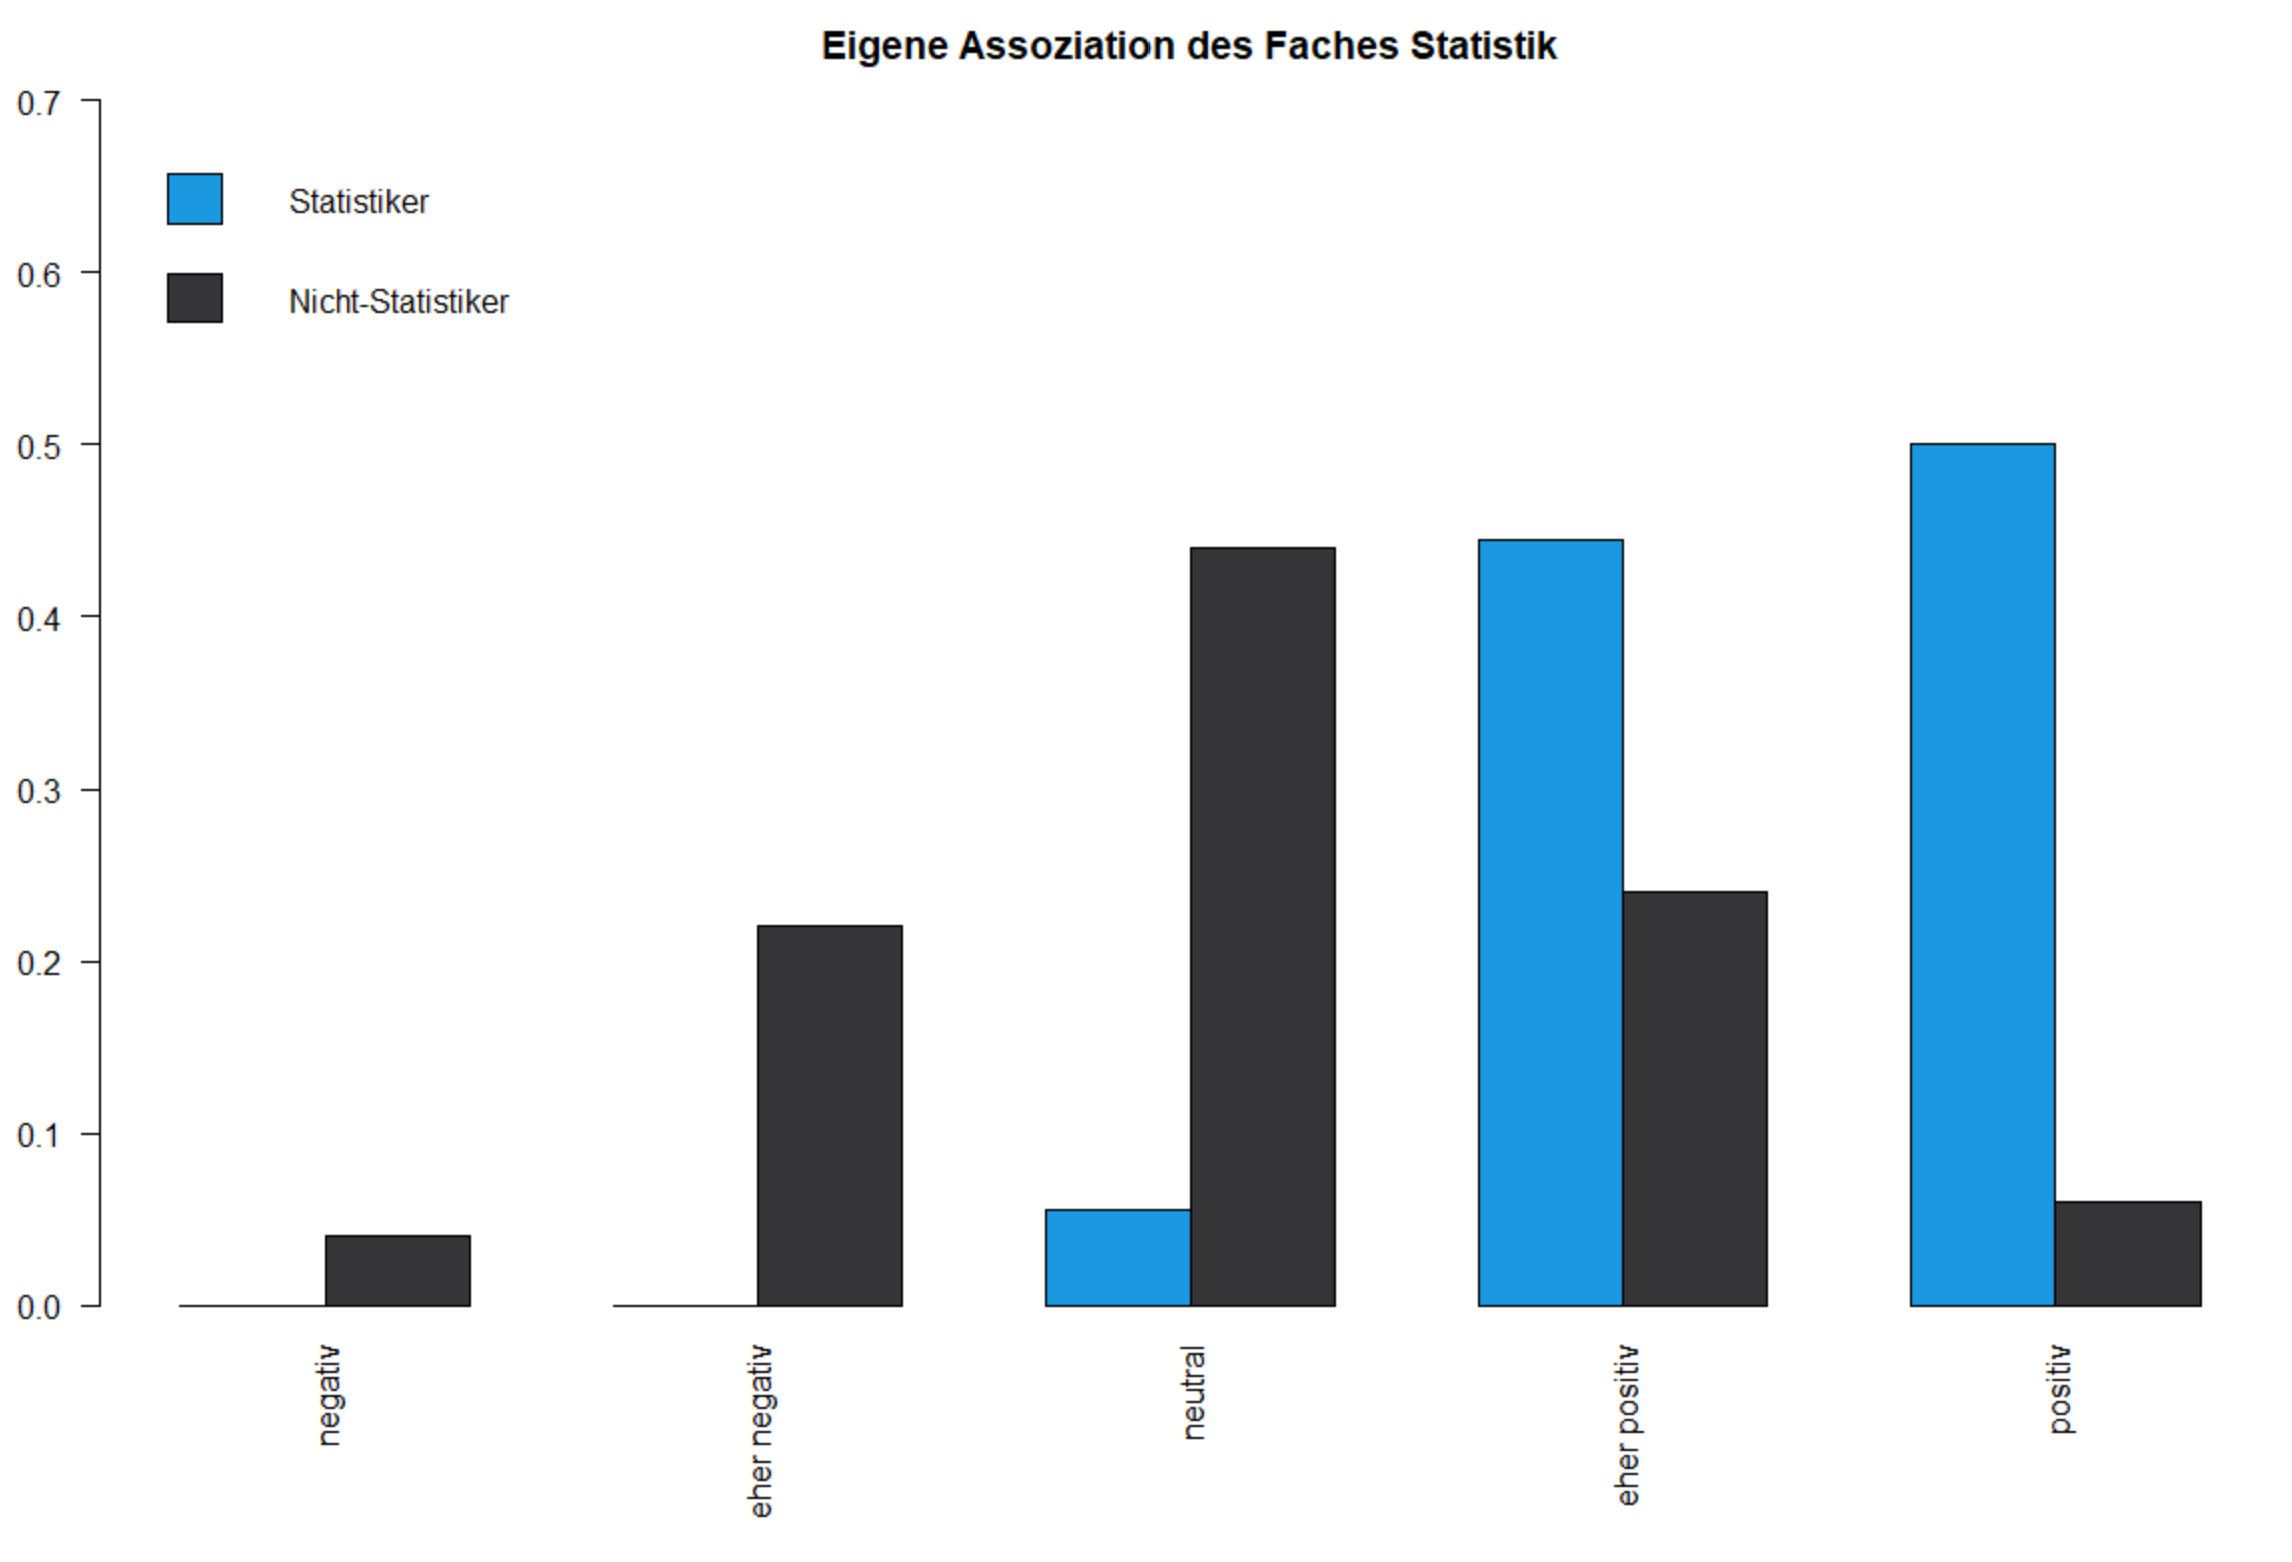
\includegraphics[scale=0.3]{(nicht)-statis_barplot_Assoziation} \\


%Wahrnehmung:\\
\hspace{-2cm}
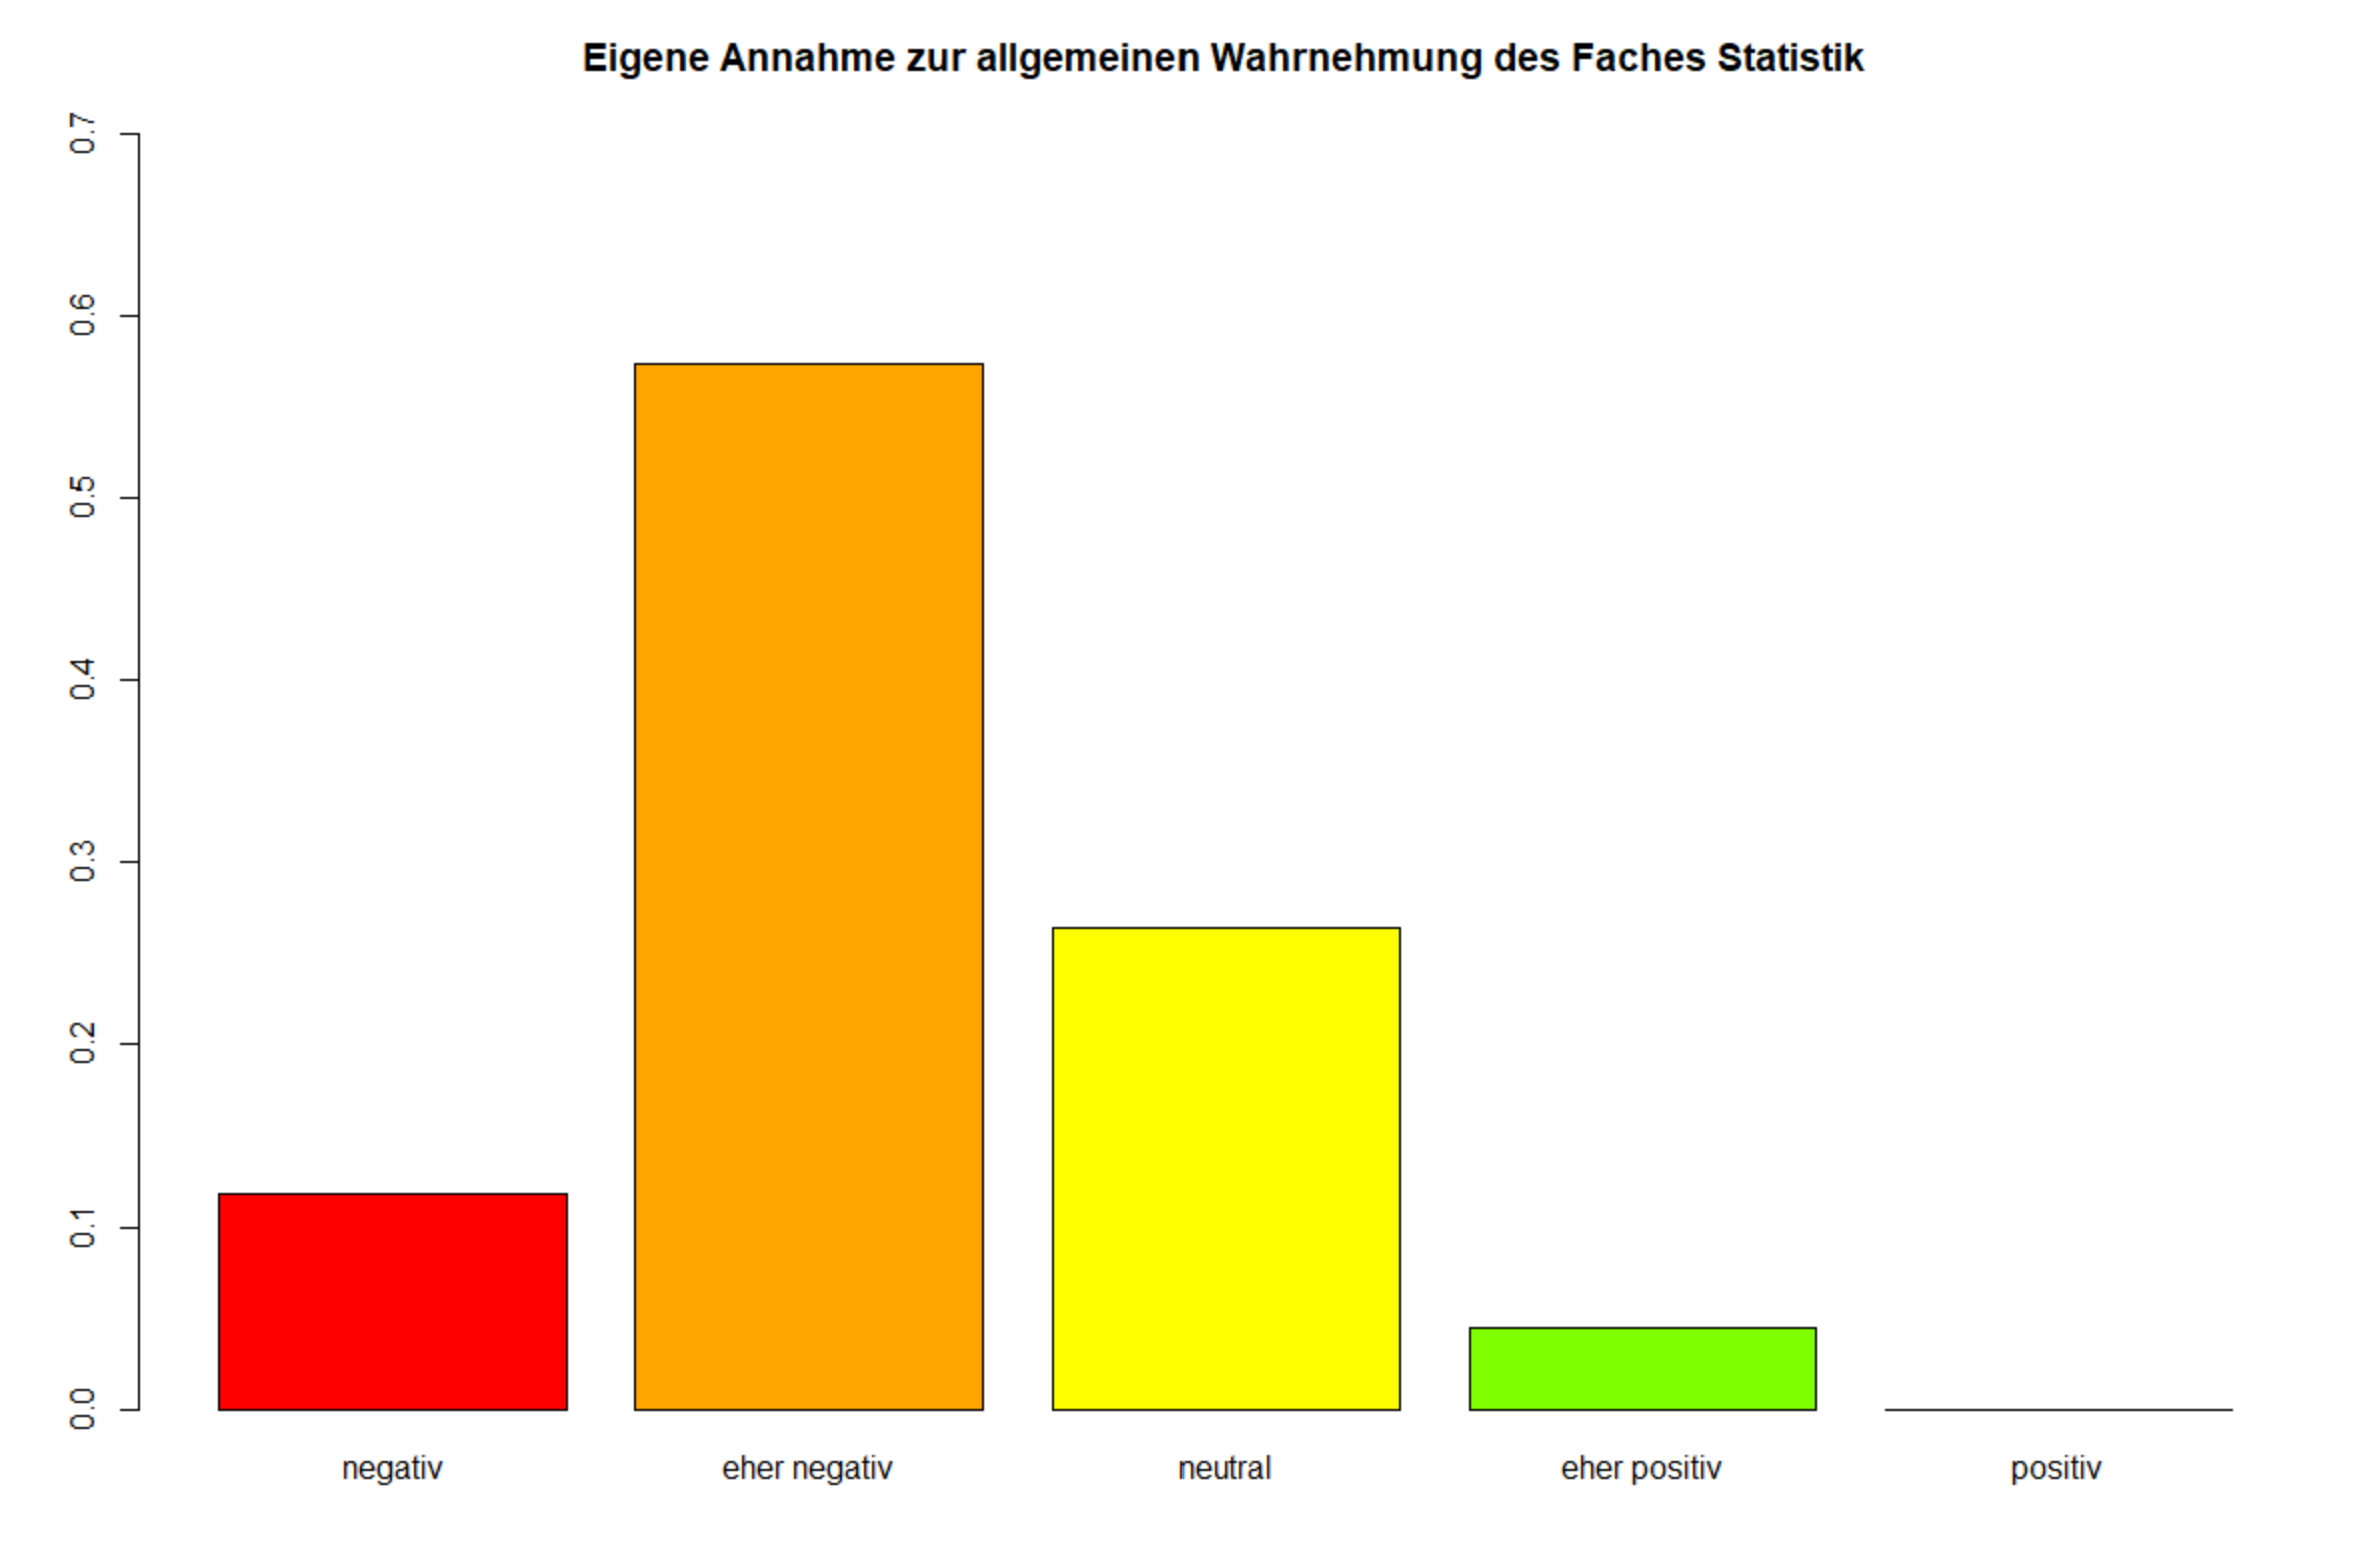
\includegraphics[scale=0.3]{barplot_Wahrnehmung}
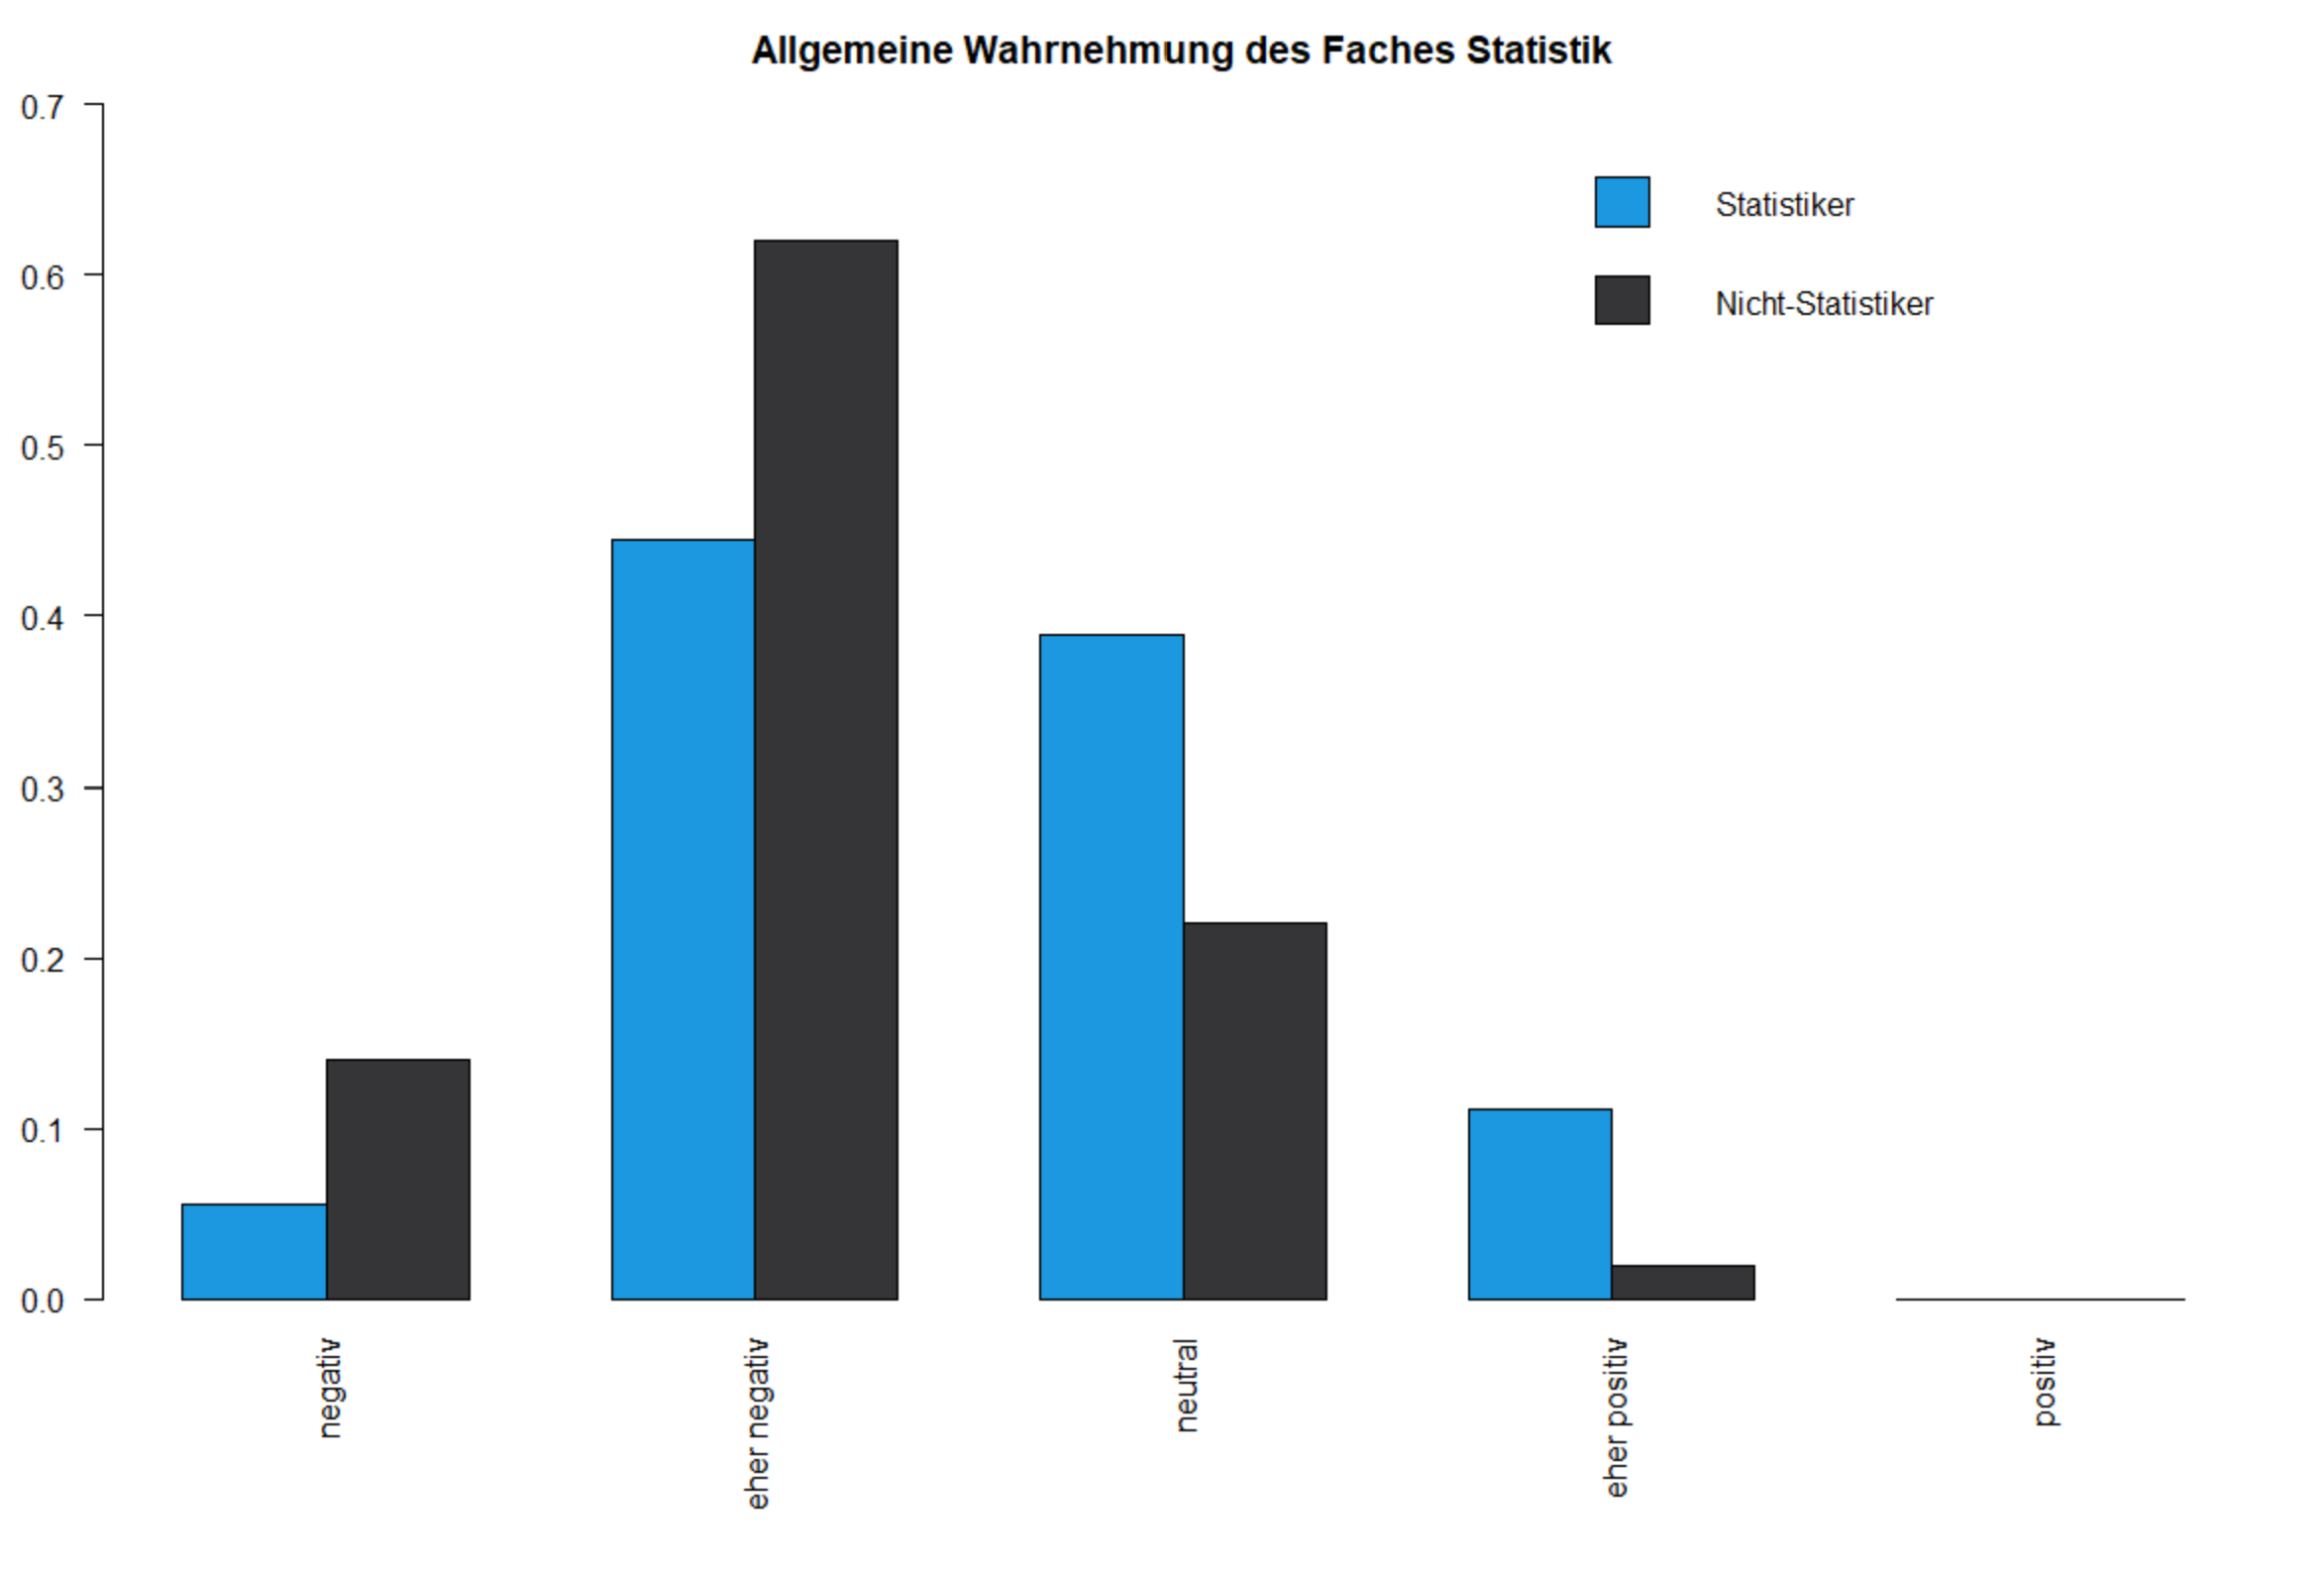
\includegraphics[scale=0.3]{(nicht)-statis_barplot_Wahrnehmung}\\

\vspace{-0.4cm}

%Text zur Forschungsfrage:\\
{\small Bis auf die Thesen \enquote{Statistiken beweisen gar nichts}, \enquote{Statistik fördert Kreativität} und \enquote{Statistik studieren nur Männer} gab es zu allen Thesen eine ziemlich eindeutige Zustimmung oder Ablehnung.\\
Negative Eigenschaften zu Beschreibung des Fachs Statistik wurden deutlich häufiger von Nicht-Statistikern angekreuzt, während die Statistiker mehr positive angekreuzt haben.\\
Besonders relevant war die Statistik für die Befragten im Studium und tendenziell im zukünftigen Beruf, jedoch weniger im Alltag. Die befragten Statistikern haben im Mittel eine höhere Relevanz für alle 3 Bereiche angegeben im Vergleich zu den Nicht-Statistikern.\\
Nicht-Statistiker haben im Mittel neutrale und Statistiker ziemlich positive Assoziationen zum Fach Statistik, was zu einer neutralen bis tendenziell positiven Assoziation im Allgemeinen führt.\\
Dennoch wird im Allgemeinen angenommen, dass die Statistik eher negativ wahrgenommen werden würde, wobei keiner der Befragten angab, dass die Wahrnehmung in der Gesellschaft \enquote{positiv} wäre.}





\end{document}